%% Companion note to "Derivation of the magnetohydrodynamic equilibrium equation"
\documentclass[english]{article}
\usepackage{mathptmx}
\renewcommand{\familydefault}{\rmdefault}
\usepackage[T1]{fontenc}
\usepackage[latin9]{inputenc}
\usepackage{geometry}
\geometry{verbose,tmargin=1in,bmargin=1in,lmargin=1in,rmargin=1in}
\usepackage{babel}
\usepackage{amsmath}
\usepackage{amssymb}
\usepackage{tikz}
\usepackage[unicode=true,pdfusetitle,
 bookmarks=true,bookmarksnumbered=false,bookmarksopen=false,
 breaklinks=false,pdfborder={0 0 1},backref=false,colorlinks=false]
 {hyperref}

\newcommand{\bB}{\mathbf{B}}
\newcommand{\bJ}{\mathbf{J}}
\newcommand{\bb}{\mathbf{b}}
\newcommand{\bv}{\mathbf{v}}
\newcommand{\br}{\mathbf{r}}
\newcommand{\bn}{\mathbf{n}}
\newcommand{\bE}{\mathbf{E}}
\newcommand{\bV}{\mathbf{V}}
\newcommand{\bI}{\mathbf{I}}
\newcommand{\gradperp}{\nabla_{\!\perp}}

\begin{document}
\title{A regularized model for 3D MHD equilibrium}
\author{Matt Landreman \& Claude Fable}
\date{July 4, 2026}
\maketitle

\begin{abstract}
The magnetohydrodynamic equilibrium model $\bJ\times\bB=\nabla p$ is pathological in generic
three-dimensional geometry: because it implies $\bB\cdot\nabla p=0$ exactly, the pressure must be
constant throughout any volume filled ergodically by a chaotic field line, and the parallel current
required by $\nabla\cdot\bJ=0$ develops $1/x$ and $\delta$-function singularities at rational
surfaces. Taking the kinetic derivation of $\bJ\times\bB=\nabla p$ in the companion
note~\cite{landreman_note} as the point of departure, we identify precisely where the assumption
of nested flux surfaces enters that derivation, and we show that the pathologies are not artifacts
of the fluid closure but theorems of the strict $\rho_*\rightarrow0$ drift-kinetic limit: at
leading order the density, temperatures, and pressure are constrained only to be invariants of the
field-line flow, a solution space that is degenerate (arbitrarily rich on a foliated field,
containing only constants on a chaotic one). The degeneracy is lifted at the next (transport) order
of the same hierarchy, where collisional entropy production first appears. Retaining these terms in
a maximal ordering yields a generalized equilibrium model in which (i)~the constraint
$\bB\cdot\nabla p=0$ is replaced by a strongly anisotropic energy-transport equation with source,
so that $p$ is smooth, non-constant, and $\bB\cdot\nabla p$ is small but nonzero; (ii)~only the
perpendicular projection of force balance, $\bJ\times\bB=\nabla p-\bb\,(\bb\cdot\nabla p)$, is
imposed, the small parallel pressure gradient being carried by the $O(\rho_*)$ anisotropic stress;
and (iii)~current continuity is closed with a small current-viscosity (hyper-resistive) flux that
replaces the singular Pfirsch--Schl\"uter and sheet currents with bounded current layers of finite
width. The result is a closed elliptic/hypoelliptic system of partial differential equations for
$(\bB,p,u=J_\parallel/B)$ that is suitable as the basis of a practical three-dimensional equilibrium
code, reduces to the classical model (and to Grad--Shafranov plus one-dimensional transport) when
nested surfaces exist, and reduces to stepped-pressure states in the vanishing-transport limit.
Alongside the predictive form of the model, in which a heating deposition is prescribed and the
profile is an output, we give an interpretive form suited to the classical workflow: a
one-dimensional pressure profile, specified as a function of enclosed volume, is realized exactly
by composing it with the level-set volume function of a reference potential that solves the same
anisotropic transport equation---requiring neither a heating source nor any tuning parameter,
while preserving the small parallel pressure gradient, island flattening, and barrier-localized
structure that the transport operator enforces.
We give the model equations, boundary conditions, input functions, an iteration scheme, recovery
checks against known analytic limits, and the relation to existing approaches
(VMEC, PIES, HINT, SPEC/MRxMHD, SIESTA, the stochastic-equilibrium analysis of
Krommes and Reiman, and the statistical equilibrium model of Ruth, Burby, Sengupta, and Brown).
\end{abstract}

\section{Overview}
\label{sec:overview}

The companion note~\cite{landreman_note} derives the magnetohydrodynamic (MHD) equilibrium
equation
\begin{equation}
\bJ\times\bB=\nabla p,
\label{eq:MHS}
\end{equation}
with $\bJ=\mu_0^{-1}\nabla\times\bB$, from the species-summed momentum moment of the
Fokker--Planck equation together with a drift-kinetic $\rho_*$ expansion, \emph{assuming good
nested flux surfaces}. The purpose of the present note is to generalize the physical model in a
principled way to non-axisymmetric three-dimensional geometry in which nested surfaces may not
exist, so that
\begin{itemize}
\item the pressure can be smooth and non-constant in regions of imperfect surfaces (magnetic
islands and field-line chaos), which requires $\bB\cdot\nabla p$ to be slightly nonzero; and
\item the parallel current density is bounded, i.e.\ the $1/x$ Pfirsch--Schl\"uter singularity and
the $\delta$-function current sheets that Eq.~(\ref{eq:MHS}) produces at rational surfaces
\cite{newcomb1959,boozer1981,cary1985,loizu2015a} are eliminated;
\end{itemize}
and to do so in a form that directly specifies the partial differential equations (PDEs) that a
practical numerical equilibrium code would solve.

The two pathologies of Eq.~(\ref{eq:MHS}) in 3D are classical. Since
$\bB\cdot(\bJ\times\bB)\equiv0$, Eq.~(\ref{eq:MHS}) implies $\bB\cdot\nabla p=0$ exactly, so $p$
is constant along field lines and hence constant on the closure of every field line. A chaotic
field line fills a volume, so $p$ must be constant throughout each chaotic region; this is Grad's
observation~\cite{grad1967} that smooth, non-constant pressure is incompatible with imperfect
surfaces. Meanwhile, the perpendicular current $\bJ_\perp=\bB\times\nabla p/B^2$ implied by
Eq.~(\ref{eq:MHS}) is generally not divergence free, and quasineutrality then forces a parallel
return current satisfying the magnetic differential equation
$\bB\cdot\nabla(J_\parallel/B)=-\nabla\cdot\bJ_\perp$, whose solutions on rational surfaces contain
a resonant $1/x$ response wherever the pressure gradient does not vanish, plus $\delta$-function
current sheets \cite{newcomb1959,boozer1981,loizu2015a,loizu2015b,helander2014}. Because the
rationals are dense, a smooth non-trivial pressure profile is essentially impossible even when
surfaces nominally exist \cite{boozer1981,grad1967}; rigorous modern results reinforce the
conclusion that solutions of Eq.~(\ref{eq:MHS}) far from symmetry are naturally piecewise-constant
in pressure with current sheets \cite{bruno1996,enciso2025,constantin2021}.

Our strategy is the following. Section~\ref{sec:recap} summarizes the derivation of the companion
note and flags the two---and only two---steps where nested surfaces are used.
Section~\ref{sec:nosurfaces} redoes those steps for a general field. The result is instructive: the
H-theorem argument \emph{survives} without any surface assumption, so the leading-order
distribution function is still a Maxwellian; what changes is that the free functions of the
leading-order solution are constrained only to be \emph{invariants of the field-line flow}. On a
foliated field the space of invariants is huge (any flux function), which is the familiar profile
freedom of equilibrium theory; on a chaotic field it collapses to constants, which is Grad's
flattening; and at rational surfaces neighboring closed lines are mutually unconstrained, which is
the origin of the current sheets. In other words, \emph{the pathologies of Eq.~(\ref{eq:MHS}) are
consequences of a degeneracy of the leading-order kinetic problem}, and any principled resolution
must invoke the next order of the same hierarchy, where the degeneracy is lifted by collisional
entropy production.

Section~\ref{sec:transport} therefore retains, in a maximal ordering, the transport-order energy
balance: the constraint $\bB\cdot\nabla p=0$ is replaced by
\begin{equation}
\nabla\cdot\Big[\kappa_\parallel\,\bb\,(\bb\cdot\nabla p)
+\kappa_\perp\big(\nabla p-\bb\,(\bb\cdot\nabla p)\big)\Big]=-S_p,
\qquad \kappa_\perp\ll\kappa_\parallel ,
\label{eq:p_preview}
\end{equation}
a uniformly elliptic anisotropic diffusion equation with heating source $S_p$, whose solutions are
smooth, non-constant, and satisfy $\bB\cdot\nabla p=O(\kappa_\perp/\kappa_\parallel)\ne0$.
Section~\ref{sec:force} shows that only the perpendicular projection of force balance,
$\bJ\times\bB=\nabla p-\bb(\bb\cdot\nabla p)$, should then be imposed---the small parallel pressure
gradient is carried by the $O(\rho_*)$ anisotropic stress---and closes current continuity with a
small ``current viscosity'' (hyper-resistive) flux,
\begin{equation}
\bB\cdot\nabla u-\nabla\cdot\big(D_u\gradperp u\big)
=\frac{2}{B^{3}}\,\bB\cdot\big(\nabla p\times\nabla B\big)
-\frac{\mu_0 u}{B^{2}}\,\bB\cdot\nabla p
+\frac{\mu_0 D_u}{B^{2}}\,\gradperp u\cdot\nabla p ,
\qquad u\equiv\frac{\bJ\cdot\bB}{B^{2}},
\label{eq:u_preview}
\end{equation}
which converts the singular resonant response into bounded current layers of width
$\propto D_u^{1/3}$ and excludes $\delta$-function sheets. Section~\ref{sec:model} assembles the
closed model and its boundary conditions and inputs, in two variants: a \emph{predictive} variant
in which the heating deposition is prescribed and the profile is an output, and an
\emph{interpretive} variant---the working mode of a classical equilibrium code, and the mode of
principal interest here---in which a one-dimensional pressure-versus-volume profile $p_0(V)$ is
prescribed directly, with neither a source nor any tuning parameter, by transplanting it onto the
level sets of a \emph{reference potential} $\chi$ generated by the same anisotropic transport
operator (Secs.~\ref{sec:transplant}--\ref{sec:Seff}). Section~\ref{sec:Vchi} describes the
accurate evaluation of the level-set volume function $V_\chi$ that this construction requires;
Sec.~\ref{sec:numerics} outlines a numerical
algorithm and verification tests; Sec.~\ref{sec:refinements} sketches the multi-species refinement
(separate $n$, $T_e$, $T_i$, and the ambipolar potential); Sec.~\ref{sec:relation} relates the
model to VMEC~\cite{hirshman1983}, PIES~\cite{reiman1986}, HINT~\cite{harafuji1989,suzuki2006},
SPEC/MRxMHD~\cite{hudson2012,qu2021}, SIESTA~\cite{hirshman2011}, and especially to the
stochastic-region equilibrium analysis of Krommes and Reiman~\cite{krommes2009}, of which the
present model can be viewed as a code-oriented, kinetically grounded packaging, as well as to the
recent statistical equilibrium model of Ruth \emph{et al.}~\cite{ruth2026}, which regularizes the
same singularities through the variance of rapid nonideal magnetic fluctuations in an averaged
variational principle;
Sec.~\ref{sec:discussion} discusses what is gained and given up.

Two remarks on scope. First, the coefficients $\kappa_\parallel$, $\kappa_\perp$, $D_u$ are
closure-level objects: their \emph{structure} (a positive-semidefinite, strongly anisotropic,
entropy-producing operator) is dictated by the kinetic hierarchy, while their precise values are
regime dependent and, in practice, partly anomalous. All macroscopic conclusions below depend only
on the structure and on the smallness of $\kappa_\perp/\kappa_\parallel$ and $D_u$, and become
insensitive to their values in the appropriate limits. Second, an unavoidable conceptual shift
accompanies the generalization: since profile information at leading order lived entirely in the
degenerate freedom of the invariants, once that degeneracy is lifted the pressure profile is no
longer a free input of the equilibrium problem but is determined by sources and transport.
``Equilibrium'' and ``transport'' cease to be separable problems in a field without surfaces. A
code can nevertheless still operate in an interpretive mode, prescribing a one-dimensional
pressure profile directly: the reference-potential construction of Sec.~\ref{sec:model} realizes a
prescribed $p_0(V)$ exactly while the transport operator retains control of \emph{where} the
isobars lie---which is the part of the profile freedom that the physics genuinely removes.

\section{Recap of the companion derivation, and where surfaces enter}
\label{sec:recap}

We use the notation of the companion note~\cite{landreman_note}. The species-summed momentum moment
of the Fokker--Planck equation gives, with quasineutrality the only approximation,
\begin{equation}
\frac{\partial}{\partial t}\Big(\sum_s m_s n_s\bV_s\Big)
=\bJ\times\bB-\nabla\cdot\Pi+\sum_s m_s\!\int d^3v\,\bv\,S_s ,
\label{eq:total_momentum}
\end{equation}
where $\Pi=\sum_s m_s\int d^3v\,\bv\bv f_s$. In the drift-kinetic ordering
($\rho_*=\rho_i/L\ll1$, low flow $V\sim\rho_* v$ as required in a general stellarator
\cite{helander2007}, $\nu\sim\rho_*\Omega$, weak sources), the time-derivative and source terms are
$O(\rho_*)$ relative to $\bJ\times\bB\sim\nabla\cdot\Pi$, so the equilibrium statement is
$\bJ\times\bB=\nabla\cdot\Pi$ at leading order, and the remaining task is to show
$\Pi\simeq p\,\bI$.

The kinetic calculation proceeds in the variables $(W_s,\mu,\vartheta)$ with
$W_s=v^2/2+q_s\Phi_0/m_s$ and $\mu=v_\perp^2/2B$. At leading order,
$\partial f_{s0}/\partial\vartheta=0$. At next order, the gyroaveraged kinetic equation reduces to
\begin{equation}
v_\parallel\,\bb\cdot\nabla f_{s0}=\overline{C_s\{f_{s0}\}} .
\label{eq:first_order}
\end{equation}
Multiplying by $(1+\ln f_{s0})$, integrating over velocity with the Jacobian appropriate to
$(W_s,\mu,\vartheta)$, and using the Leibniz-rule/$\sigma$-summation argument of the companion note
to pull $\bB\cdot\nabla$ outside the velocity integrals, one obtains the \emph{pointwise} identity
\begin{equation}
\bB\cdot\nabla Y_s(\br)=\int d^3v\,\ln f_{s0}\,C_s\{f_{s0}\},
\qquad
Y_s\equiv\sum_\sigma\sigma\int_0^{2\pi}\!\!d\vartheta\int_0^\infty\!\!d\mu
\int_{\mu B+q_s\Phi_0/m_s}^{\infty}\!\!dW_s\,f_{s0}\ln f_{s0}.
\label{eq:pointwise_entropy}
\end{equation}
The derivation then invokes nested surfaces exactly twice:
\begin{itemize}
\item[{[S1]}] The flux-surface average is applied to Eq.~(\ref{eq:pointwise_entropy}); since
$\langle\bB\cdot\nabla w\rangle=0$ for single-valued $w$, the left side is annihilated, and the
H-theorem inequality $\int d^3v\,\ln f_{s0}\,C_s\{f_{s0}\}\le0$ then forces the integrand to vanish
pointwise, so $f_{s0}$ is a local Maxwellian.
\item[{[S2]}] With $C_s\{f_{s0}\}=0$, Eq.~(\ref{eq:first_order}) gives
$v_\parallel\bb\cdot\nabla f_{s0}=0$, whence $V_{s0}=0$, $\bb\cdot\nabla T_s=0$, and
$\bb\cdot\nabla N_s=0$; the conclusion $T_s=T_s(\psi)$, $N_s=N_s(\psi)$ (and, via quasineutrality,
$\Phi_0=\Phi_0(\psi)$, $n_s=n_s(\psi)$) uses the fact that a quantity constant along field lines
that cover nested surfaces is a flux function.
\end{itemize}
With $f_{s0}$ a stationary isotropic Maxwellian, $\Pi=p\,\bI$ with $p=\sum_s n_sT_s$, and
Eq.~(\ref{eq:total_momentum}) yields Eq.~(\ref{eq:MHS}). We now revisit [S1] and [S2] for a general
three-dimensional field.

\section{The derivation without nested flux surfaces}
\label{sec:nosurfaces}

\subsection{Invariant sets and the generalized annihilator}
\label{sec:annihilator}

Let $\Omega$ be the plasma region, and consider the fixed-boundary problem in which
$\bB\cdot\hat{\bn}=0$ on $\partial\Omega$ (the free-boundary case is deferred to
Sec.~\ref{sec:model}). Call an open set $\Omega'\subseteq\Omega$ \emph{invariant} if
$\bB\cdot\hat{\bn}=0$ on $\partial\Omega'$, i.e.\ if its boundary is composed of field lines and
invariant surfaces. For any single-valued, integrable $w(\br)$ and any invariant $\Omega'$,
\begin{equation}
\int_{\Omega'} d^3r\;\bB\cdot\nabla w
=\int_{\Omega'} d^3r\;\nabla\cdot(w\bB)
=\oint_{\partial\Omega'} dA\;w\,\bB\cdot\hat{\bn}=0 .
\label{eq:annihilator}
\end{equation}
Equation~(\ref{eq:annihilator}) is the generalization of $\langle\bB\cdot\nabla w\rangle=0$: the
flux-surface average is the special case in which $\Omega'$ is the thin shell between two
neighboring invariant tori. When nested surfaces do not exist, invariant sets still do: the whole
plasma $\Omega$ itself; regions foliated by KAM tori; island regions bounded by their separatrices;
and each connected chaotic component, whose boundary consists of bounding KAM surfaces, separatrices,
or the wall. (Cantori, being invariant sets of measure zero with gaps, do \emph{not} bound invariant
open sets; a single chaotic component may be partitioned by cantori into subregions connected
through turnstiles \cite{meiss1992}, but it remains one transitive component. This distinction
becomes important, and useful, at transport order.)

\subsection{The Maxwellian survives; step [S1] needs no surfaces}
\label{sec:maxwellian}

Apply Eq.~(\ref{eq:annihilator}) with $w=Y_s$ and $\Omega'=\Omega$ to
Eq.~(\ref{eq:pointwise_entropy}):
\begin{equation}
\int_\Omega d^3r\int d^3v\,\ln f_{s0}\,C_s\{f_{s0}\}=0 .
\end{equation}
By the H-theorem the integrand is nonpositive everywhere, so it vanishes almost everywhere, and the
same argument as in the companion note gives that $f_{s0}$ is a local Maxwellian
\emph{throughout $\Omega$, with no assumption whatsoever about the internal structure of the field}.
(The multi-species subtleties---whether the temperatures of different species are forced equal by
inter-species collisions or are treated separately---are exactly as discussed in the companion note
and do not affect what follows.) This is a mild strengthening of [S1]: the only geometric input is
that the outer boundary is a flux surface. The leading-order stress is therefore isotropic,
$\Pi_0=p\,\bI$, in complete generality.

\subsection{Step [S2] becomes a statement about invariants of the field-line flow}
\label{sec:invariants}

With $f_{s0}$ Maxwellian, $C_s\{f_{s0}\}=0$ and Eq.~(\ref{eq:first_order}) again gives
$v_\parallel\bb\cdot\nabla f_{s0}=0$. The velocity-space decomposition performed in the companion
note goes through verbatim---it is entirely local in $\br$---and yields
\begin{equation}
V_{s0}=0,\qquad \bb\cdot\nabla T_s=0,\qquad \bb\cdot\nabla N_s=0 ,
\label{eq:parallel_constraints}
\end{equation}
where $N_s=n_s\exp(q_s\Phi_0/T_s)$ is the pseudo-density. (The proof that $V_{s0}=0$ used only
$\bb\cdot\nabla B\ne0$ almost everywhere, which holds in any toroidal plasma.) The quasineutrality
argument of the companion note likewise localizes: at each point,
$N_i/N_e=\exp\big(e\Phi_0/T_e+e\Phi_0/T_i\big)$ for a hydrogenic plasma, so $\bb\cdot\nabla$ of the
left side vanishing forces $\bb\cdot\nabla\Phi_0=0$ and hence $\bb\cdot\nabla n_s=0$ and
$\bb\cdot\nabla p=0$.

Thus the correct general statement replacing ``$T_s$, $N_s$, $\Phi_0$, $n_s$, $p$ are flux
functions'' is:
\begin{quote}
\emph{At leading order in $\rho_*$, the profiles $T_s$, $N_s$, $\Phi_0$, $n_s$, and $p$ are
continuous invariants of the field-line flow: they are constant on the closure of every field
line.}
\end{quote}
Everything that is right and everything that is pathological about three-dimensional MHD
equilibrium follows from the structure of this space of invariants, $\mathcal{I}(\bB)$, on the
ergodic partition of the field:
\begin{enumerate}
\item \textbf{Regions foliated by nested tori.} Almost every line is dense in its torus, so an
invariant is a function of the surface label alone: $p=p(\psi)$, etc. The classical picture is
recovered, including its familiar \emph{profile freedom}: any $p(\psi)$ is admissible at this
order.
\item \textbf{Island chains.} The same statement holds with respect to the island's own nested
surfaces: invariants are functions of the island surface label. In particular $p$ takes a single
value on each island flux surface, and its value at the island O-point is unrelated, at this order,
to the profile outside the separatrix.
\item \textbf{Chaotic components.} A chaotic component $\Omega_c$ is topologically transitive: some
field line is dense in $\Omega_c$. A continuous invariant is therefore \emph{constant throughout}
$\Omega_c$:
\begin{equation}
p=\text{const},\quad T_s=\text{const},\quad n_s=\text{const}\quad\text{on each chaotic component.}
\label{eq:flattening}
\end{equation}
This is Grad's flattening obstruction \cite{grad1967}, here derived from the drift-kinetic
hierarchy rather than postulated from the fluid model. Note that partial barriers (cantori) offer
no protection at this order: however long the transit time through a turnstile, the invariance
constraint is exact, and the component supports no gradient. Gradients across cantori can only be
recovered by physics beyond leading order.
\item \textbf{Rational surfaces.} On a rational torus every line closes on itself; each closed line
is its own ergodic set. Continuity forces the invariants to be constant on the torus (the limits
from the neighboring irrational tori pinch them), but nothing at this order relates the
\emph{one-sided derivatives}: the profiles $p(\psi)$, $T_s(\psi)$ may have kinks at every rational
surface. This is precisely the freedom that the current-continuity constraint exploits and that
generates singular current sheets, as we now recall.
\end{enumerate}

\subsection{Current continuity and the two singularities}
\label{sec:singular_currents}

Write $\bJ=u\bB+\bJ_\perp$ with $u=\bJ\cdot\bB/B^2$ and, from Eq.~(\ref{eq:MHS}),
$\bJ_\perp=\bB\times\nabla p/B^2$. Using $\nabla\cdot(\mathbf{F}\times\mathbf{G})
=\mathbf{G}\cdot\nabla\times\mathbf{F}-\mathbf{F}\cdot\nabla\times\mathbf{G}$ with
$\mathbf{F}=\bB/B^2$ and $\mathbf{G}=\nabla p$,
\begin{equation}
\nabla\cdot\bJ_\perp
=\nabla p\cdot\nabla\times\!\Big(\frac{\bB}{B^{2}}\Big)
=\frac{\mu_0\,\bJ\cdot\nabla p}{B^{2}}
-\frac{2}{B^{3}}\,\bB\cdot\big(\nabla p\times\nabla B\big) ,
\label{eq:divJperp}
\end{equation}
and quasineutrality $\nabla\cdot\bJ=0$ with $\nabla\cdot(u\bB)=\bB\cdot\nabla u$ gives, in the
classical model where $\bB\cdot\nabla p=0$ (so $\bJ\cdot\nabla p=0$), the magnetic differential
equation (MDE)
\begin{equation}
\bB\cdot\nabla u=\frac{2}{B^{3}}\,\bB\cdot\big(\nabla p\times\nabla B\big)\equiv h .
\label{eq:MDE}
\end{equation}
Where straight-field-line coordinates $(\psi,\theta,\varphi)$ exist,
$\bB\cdot\nabla\,e^{i(m\theta-n\varphi)}\propto i\,(m\iota-n)\,e^{i(m\theta-n\varphi)}$, and the
Fourier solution $u_{mn}\propto h_{mn}/(m\iota-n)$ exhibits the two well-known pathologies
\cite{newcomb1959,boozer1981,loizu2015a,loizu2015b,helander2014}: (i)~a resonant
\emph{Pfirsch--Schl\"uter} response $u_{mn}\propto 1/x$ near a surface where $\iota=n/m$, with
$x$ the distance from the surface, whenever the resonant harmonic $h_{mn}$---which is proportional
to the local $p'$---does not vanish there; solvability in the sense of Newcomb requires
$h_{mn}=0$ on the resonant surface, which for generic geometry forces $p'=0$ there
\cite{newcomb1959,boozer1981,cary1985}; and (ii)~$\delta$-function current sheets, the homogeneous
solutions supported on rational surfaces, which are required if the response is to remain ideal
(island-shielding) \cite{loizu2015a,loizu2015b}. Since the rationals are dense, requirement~(i)
alone already forbids a smooth profile with $p'\ne0$ on any interval \cite{boozer1981,grad1967};
the rigorous constructions of three-dimensional equilibria far from symmetry accordingly carry
piecewise-constant pressure and current sheets \cite{bruno1996,enciso2025}, and smooth
non-symmetric solutions of Eq.~(\ref{eq:MHS}) with nontrivial pressure are, at best, highly
exceptional \cite{constantin2021}.

\subsection{Diagnosis: a degenerate leading order}
\label{sec:diagnosis}

The picture that emerges is coherent. The leading-order drift-kinetic problem determines the
\emph{form} of $f_{s0}$ (Maxwellian) everywhere, but determines the profiles only up to an
arbitrary element of $\mathcal{I}(\bB)$. That solution space is degenerate in a way that depends
discontinuously on the field: on a foliated field it is an infinite-dimensional family (all flux
functions), on a chaotic component it is one-dimensional (constants), and across the dense set of
rational surfaces its elements may be glued non-smoothly. The classical equilibrium problem tries
to select a member of this space using only the leading-order momentum equation---i.e., using
$\bB\cdot\nabla p=0$, which is nothing but the statement $p\in\mathcal{I}(\bB)$---and therefore
inherits the degeneracy as profile freedom, flattening, and current sheets, depending on where one
looks.

Physically, the member of $\mathcal{I}(\bB)$ that nature selects is determined by the next order of
the hierarchy: the transport time scale, on which collisional entropy production first appears and
on which sources and sinks compete with cross-field fluxes. On a foliated field this selection is
familiar---it is one-dimensional neoclassical/anomalous transport across surfaces, conventionally
solved as a separate ``transport problem'' after the equilibrium is computed. Without a foliation
the two problems cannot be separated: the transport-order terms are the \emph{largest terms in the
hierarchy that are not degenerate on $\mathcal{I}(\bB)$}, and they must be retained inside the
equilibrium model itself. That is the generalization we now construct. The two limits
$\rho_*\rightarrow0$ and $t\rightarrow\infty$ do not commute in a chaotic region, and the classical
model corresponds to taking $\rho_*\rightarrow0$ first.

\section{Lifting the degeneracy: the transport-order pressure equation}
\label{sec:transport}

\subsection{Subsidiary ordering}
\label{sec:ordering}

Within the ordering of the companion note ($\nu\sim\rho_*\Omega$), the collisional parallel and
perpendicular heat diffusivities scale as
\begin{equation}
\chi_\parallel\sim\frac{v_t^{2}}{\nu}=v_t\lambda,
\qquad
\chi_\perp^{\rm (cl)}\sim\nu\rho^{2},
\qquad
\varepsilon_\kappa\equiv\frac{\chi_\perp}{\chi_\parallel}
\sim\Big(\frac{\nu}{\Omega}\Big)^{2}\sim\rho_*^{2},
\label{eq:epsilon_kappa}
\end{equation}
with $\lambda=v_t/\nu$ the mean free path. (Parallel conduction is dominated by electrons,
perpendicular collisional conduction by ions, and in practice $\chi_\perp$ is enhanced by
neoclassical geometry and by turbulence to anomalous values; all of this only \emph{increases}
$\varepsilon_\kappa$ while leaving it very small, typically
$\varepsilon_\kappa\sim10^{-10}$--$10^{-6}$ across the channels and regimes of a fusion-grade
plasma \cite{braginskii1965,helander_sigmar}.) Transport thus enters two orders in $\rho_*$ below
the terms retained at leading order---which is why it was invisible in
Sec.~\ref{sec:nosurfaces}---but it is the largest effect that distinguishes among the members of
$\mathcal{I}(\bB)$. A maximal ordering that resolves the degeneracy therefore keeps
$\varepsilon_\kappa$ finite in the energy balance while continuing to drop $O(\rho_*)$ corrections
to force balance itself. Mixed-order truncations of this kind are standard in transport theory
(force balance holds at each instant at leading order; profiles are governed by transport-order
balances); the only novelty here is that the transport-order balance must be solved as a
three-dimensional PDE rather than flux-surface averaged to one dimension.

\subsection{Energy balance and closure}
\label{sec:energy}

Take the $m_sv^2/2$ moment of the kinetic equation, sum over species (collisional energy exchange
cancels in the sum), and use steady state:
\begin{equation}
\nabla\cdot\mathbf{Q}=\bJ\cdot\bE+S_E,
\qquad
\mathbf{Q}\equiv\sum_s\frac{m_s}{2}\int d^3v\,v^{2}\bv f_s ,
\label{eq:energy_moment}
\end{equation}
with $S_E$ the net heating power density (external heating minus radiation, etc.). In a static
state $\bE=-\nabla\Phi$, and $\nabla\cdot\bJ=0$ gives $\bJ\cdot\bE=-\nabla\cdot(\Phi\bJ)$, so with
$\mathbf{q}\equiv\mathbf{Q}+\Phi\bJ$,
\begin{equation}
\nabla\cdot\mathbf{q}=S_E .
\label{eq:energy_conservation}
\end{equation}
Equation~(\ref{eq:energy_conservation}) is exact (given quasineutrality and steady state). The
closure step is to evaluate $\mathbf{q}$ from the kinetic solution: $f_{s0}$ contributes the
convective flux $\sum_s\tfrac{5}{2}p_s\bV_s$ (transport order, since $V\sim\rho_*v$); the
first-order correction $f_{s1}$ contributes the parallel conductive flux
$\propto-\kappa_\parallel\bb\,\bb\cdot\nabla T$ and diamagnetic heat flows whose divergences
supply the geometric (Pfirsch--Schl\"uter--type) contributions; and second-order/collisional
finite-Larmor-radius corrections supply the classical perpendicular conduction. We adopt the
standard model closure
\begin{equation}
\mathbf{q}=-\,\kappa_\parallel\,\bb\,(\bb\cdot\nabla T)
-\,\kappa_\perp\big(\nabla T-\bb\,(\bb\cdot\nabla T)\big)+\cdots ,
\label{eq:q_closure}
\end{equation}
and emphasize which of its features are essential and which are conventional. Essential are three
structural properties inherited from the kinetic hierarchy: (P1)~strong anisotropy,
$\kappa_\perp/\kappa_\parallel=\varepsilon_\kappa\ll1$; (P2)~a positive-semidefinite conductivity,
so that the associated entropy production
$\int d^3r\,[\kappa_\parallel(\bb\cdot\nabla T)^{2}+\kappa_\perp|\gradperp T|^{2}]/T^{2}\ge0$ has
the sign guaranteed by the H-theorem at this order (cf.\ the role of entropy production in relaxed
states \cite{hameiri1987}); and (P3)~reduction, on nested surfaces and after flux-surface
averaging, to the standard one-dimensional radial transport law with the appropriate
neoclassical/anomalous $\kappa_\perp$ \cite{helander_sigmar}. Conventional is the local Fourier
form of the parallel term: in the long-mean-free-path regime the true parallel response is
nonlocal, and Eq.~(\ref{eq:q_closure}) with a (possibly flux-limited,
$\kappa_\parallel\lesssim\alpha\,n v_t L_c$) coefficient is a surrogate whose only essential
property here is that it relaxes $T$ toward constancy along field lines on connection-length
scales. Any closure with properties (P1)--(P3) produces the same macroscopic structure below.

For the \emph{minimal} model we collapse the species and channels into a single equation for the
total pressure, absorbing convective and drift contributions into effective coefficients:
\begin{equation}
\boxed{\;
\nabla\cdot\Big[\kappa_\parallel\,\bb\,(\bb\cdot\nabla p)
+\kappa_\perp\big(\nabla p-\bb\,(\bb\cdot\nabla p)\big)\Big]=-\,S_p ,
\qquad p=p_b\;\text{on}\;\partial\Omega .
\;}
\label{eq:pressure_equation}
\end{equation}
Here $\kappa_{\parallel,\perp}$ are pressure diffusivities (possibly functions of position and of
the fields) and $S_p\ge0$ is the pressure source corresponding to the heating deposition profile.
A production code would instead evolve $n$, $T_e$, $T_i$ separately with particle sources and
inter-species exchange (Sec.~\ref{sec:refinements}); nothing below depends on this simplification.

\subsection{Properties of the pressure equation}
\label{sec:p_properties}

\paragraph{Well-posedness, smoothness, positivity.}
The conductivity tensor
$K=\kappa_\perp\bI+(\kappa_\parallel-\kappa_\perp)\bb\bb$ has eigenvalues
$\{\kappa_\parallel,\kappa_\perp,\kappa_\perp\}$, so for $\kappa_\perp>0$
Eq.~(\ref{eq:pressure_equation}) is uniformly elliptic, however extreme the anisotropy. Its weak
solutions are the unique minimizers of
\begin{equation}
\mathcal{F}[p]=\int_\Omega\Big[\tfrac12\kappa_\parallel(\bb\cdot\nabla p)^{2}
+\tfrac12\kappa_\perp\big|\gradperp p\big|^{2}-S_p\,p\Big]\,d^3r ,
\qquad p=p_b\ \text{on}\ \partial\Omega ,
\label{eq:variational}
\end{equation}
which exists and is unique by coercivity (Lax--Milgram); for smooth $\bB$, $\kappa$'s and $S_p$,
elliptic regularity makes $p$ smooth in the interior; and the maximum principle with $S_p\ge0$
gives $p\ge\min p_b>0$ and places the maximum of $p$ in the source region. \emph{Smooth,
positive pressure is thus guaranteed by construction, for any field-line topology.} Non-constancy
is equally automatic wherever heat must flow: integrating Eq.~(\ref{eq:pressure_equation}) over the
volume inside any closed surface $\Sigma$ enclosing net heating power $P_\Sigma>0$ gives
$\oint_\Sigma(K\nabla p)\cdot\hat{\bn}\,dA=-P_\Sigma$, so $\nabla p\ne0$ somewhere on every such
surface---including surfaces threading chaotic regions. The requested behavior---smooth,
non-constant pressure across regions of imperfect surfaces---is therefore not merely permitted but
enforced.

\paragraph{$\bB\cdot\nabla p$ is small but nonzero.}
In steady state the divergences of the parallel and perpendicular fluxes balance each other and the
source, so on structures with parallel connection length $L_\parallel$ and transverse scale
$L_\perp$,
\begin{equation}
\frac{|\bb\cdot\nabla p|}{|\gradperp p|}
\sim\varepsilon_\kappa\,\frac{L_\parallel}{L_\perp},
\label{eq:Bdotgradp_estimate}
\end{equation}
which for $\varepsilon_\kappa\sim10^{-10}$--$10^{-6}$ is minute yet strictly nonzero: exactly the
``slightly nonzero $\bB\cdot\nabla p$'' the generalized model is meant to allow. In the formal
limit $\varepsilon_\kappa\rightarrow0$ on a foliated field, $\bb\cdot\nabla p\rightarrow0$ and
$p\rightarrow p(\psi)$, recovering the classical constraint as the leading term of a regular
expansion rather than as an exact degenerate equation.

\paragraph{Recovered limits.}
The single equation~(\ref{eq:pressure_equation}) contains, in the appropriate limits, the known
analytic results for every type of field region:
\begin{enumerate}
\item \emph{Nested surfaces.} Writing $p=\bar p(\psi)+O(\varepsilon_\kappa)$ and flux-surface
averaging Eq.~(\ref{eq:pressure_equation}) annihilates the parallel term and yields the standard
one-dimensional transport equation
\begin{equation}
\frac{1}{V'}\frac{d}{d\psi}\Big[V'\big\langle\kappa_\perp|\nabla\psi|^{2}\big\rangle
\frac{d\bar p}{d\psi}\Big]=-\langle S_p\rangle ,
\label{eq:1D_transport}
\end{equation}
so the classical ``free function'' $p(\psi)$ is selected by sources and $\kappa_\perp$---the
equilibrium and transport problems merge, as they must (Sec.~\ref{sec:diagnosis}).
\item \emph{An isolated island chain.} Equation~(\ref{eq:pressure_equation}) linearized about a
resonant layer is precisely the boundary-layer problem analyzed by Fitzpatrick
\cite{fitzpatrick1995}: with magnetic shear length $L_s$ and resonant wavenumber $k_\theta$, the
parallel wavenumber a distance $w$ from the rational surface is $k_\parallel\sim k_\theta w/L_s$,
and balancing $\chi_\parallel k_\parallel^{2}\sim\chi_\perp/w^{2}$ gives the critical width
\begin{equation}
w_c\sim\Big(\frac{\chi_\perp}{\chi_\parallel}\Big)^{1/4}
\Big(\frac{L_s}{k_\theta}\Big)^{1/2}
=\varepsilon_\kappa^{1/4}\Big(\frac{L_s}{k_\theta}\Big)^{1/2}.
\label{eq:wc}
\end{equation}
Islands wider than $w_c$ flatten $p$ across their interior; islands narrower than $w_c$ leave the
profile essentially unperturbed. Because island widths shrink rapidly with mode number while $w_c$
is fixed by $\varepsilon_\kappa$, only a finite set of low-order resonances imprint visible
features: \emph{the dense-rationals pathology of Sec.~\ref{sec:singular_currents} is resolved by a
physical cutoff}, and $p$ is smooth with a finite number of localized gradient depressions.
\item \emph{Chaotic regions.} With $\bb$ chaotic, the operator
$\kappa_\parallel(\bb\cdot\nabla)^{2}$ transports heat along stochastically wandering lines and,
upon coarse-graining, produces the enhanced effective cross-field transport familiar from
stochastic-field transport theory \cite{rechester1978}; the residual gradients concentrate on the
partial barriers (cantori and island remnants), where field-line transport is slow. This is the
regime computed by Hudson and Breslau \cite{hudson2008}, whose steady-state isotherms of
Eq.~(\ref{eq:pressure_equation}) (without source) track the ``ghost surfaces'' of the chaotic
field, and analyzed rigorously by Helander, Hudson and Paul \cite{helander2022,paul2022}, who
bound the temperature variation along $\bB$ and quantify the effective non-integrable volume. In
the present model these results describe the interior structure of the equilibrium pressure
itself: $p$ is smooth, decreasing on average across the chaotic annulus at the rate required to
carry the heating power through it, with its gradient localized at the surviving barriers.
\item \emph{The vanishing-transport limit.} As $\varepsilon_\kappa\rightarrow0$ with a chaotic
region present, the solution of Eq.~(\ref{eq:pressure_equation}) tends toward a function constant
on each chaotic component with jumps concentrated at the bounding KAM surfaces---i.e., toward the
stepped-pressure states of MRxMHD/SPEC \cite{hudson2012}. The classical pathologies and the
stepped-pressure resolution both appear as singular limits of the transport-regularized model
(Fig.~\ref{fig:profiles}).
\end{enumerate}

\begin{figure}[tb]
\centering
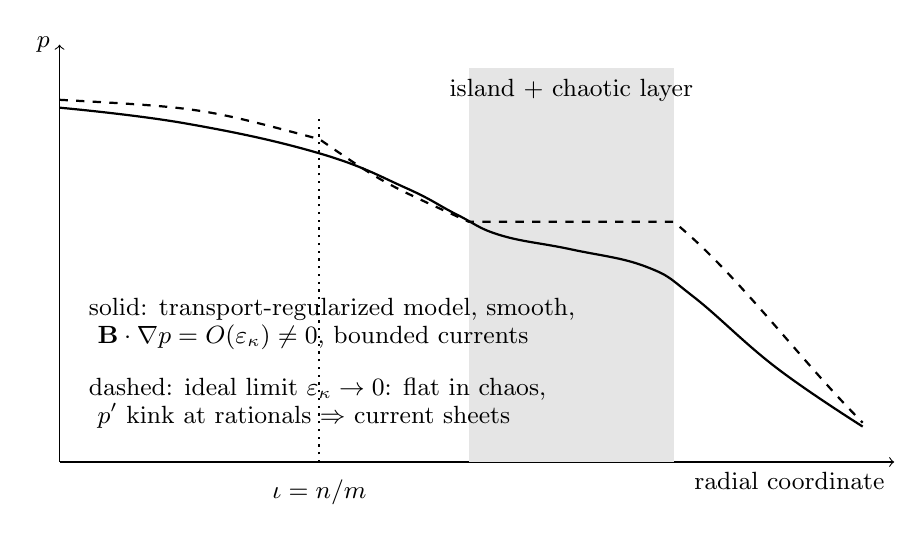
\begin{tikzpicture}[scale=1.0]
\draw[->] (0,0) -- (10.6,0) node[below left] {\small radial coordinate};
\draw[->] (0,0) -- (0,5.3) node[left] {\small $p$};
\fill[black!10] (5.2,0) rectangle (7.8,5.0);
\node at (6.5,4.72) {\small island $+$ chaotic layer};
\draw[dotted,thick] (3.3,0) -- (3.3,4.35);
\node at (3.3,-0.38) {\small $\iota=n/m$};
\draw[dashed,thick]
 (0,4.6) .. controls (1.8,4.5) .. (3.3,4.1)
 .. controls (4.1,3.55) .. (5.2,3.05)
 -- (7.8,3.05)
 .. controls (8.6,2.4) and (9.4,1.3) .. (10.2,0.5);
\draw[thick]
 plot[smooth,tension=0.7] coordinates {(0,4.5) (1.6,4.3) (3.3,3.92) (4.4,3.48)
 (5.05,3.14) (5.6,2.88) (6.5,2.7) (7.45,2.48) (8.05,2.1) (9.1,1.2) (10.2,0.45)};
\node[align=left,anchor=west] at (0.25,1.75)
 {\small solid: transport-regularized model, smooth,\\[-2pt]
  \small \ $\bB\cdot\nabla p=O(\varepsilon_\kappa)\neq0$, bounded currents};
\node[align=left,anchor=west] at (0.25,0.75)
 {\small dashed: ideal limit $\varepsilon_\kappa\rightarrow0$: flat in chaos,\\[-2pt]
  \small \ $p'$ kink at rationals $\Rightarrow$ current sheets};
\end{tikzpicture}
\caption{Schematic pressure profiles across a region containing a low-order rational surface and an
island/chaotic layer. In the ideal limit (dashed), the pressure is exactly flat across the chaotic
component, and its derivative is discontinuous at rational surfaces, sourcing $1/x$ and
$\delta$-function parallel currents. In the transport-regularized model (solid), the profile is
smooth everywhere; gradients survive at partial barriers (cantori, island remnants) and are
depressed, over the width $\max(w_{\rm island},w_c)$ with $w_c\propto\varepsilon_\kappa^{1/4}$, at
low-order resonances, which simultaneously removes the drive for the singular currents.}
\label{fig:profiles}
\end{figure}

\section{Force balance and current continuity with $\bB\cdot\nabla p\neq0$}
\label{sec:force}

\subsection{Which projection of the momentum equation to impose}
\label{sec:projection}

Since $\bB\cdot(\bJ\times\bB)\equiv0$, Eq.~(\ref{eq:MHS}) cannot be imposed verbatim once
$\bB\cdot\nabla p\ne0$: the classical equation over-constrains the system by exactly the degenerate
relation $p\in\mathcal{I}(\bB)$ diagnosed in Sec.~\ref{sec:diagnosis}. The resolution is dictated
by the ordering of the exact momentum balance~(\ref{eq:total_momentum}). Writing
$\Pi=p\,\bI+\pi$, where $\pi=O(\rho_*)\,p$ collects the gyroviscous, parallel-viscous
(pressure-anisotropy), and perpendicular-viscous stresses generated at first order,
the two projections of $0=\bJ\times\bB-\nabla p-\nabla\cdot\pi+O(\rho_*^{2})$ are:
\begin{align}
\text{perpendicular:}\qquad &
\bJ\times\bB=\nabla p-\bb\,(\bb\cdot\nabla p)
+\big[\nabla\cdot\pi\big]_\perp ,
\label{eq:perp_balance}\\
\text{parallel:}\qquad &
0=\bb\cdot\nabla p+\bb\cdot(\nabla\cdot\pi) .
\label{eq:par_balance}
\end{align}
The generalized model imposes Eq.~(\ref{eq:perp_balance}) at leading order,
\begin{equation}
\bJ\times\bB=\nabla p-\bb\,(\bb\cdot\nabla p)\equiv\gradperp p ,
\label{eq:perp_model}
\end{equation}
and treats Eq.~(\ref{eq:par_balance}) as a higher-order relation that determines the small
anisotropic stress a posteriori rather than as a constraint on $p$: since
$\bb\cdot\nabla p\sim\varepsilon_\kappa\,p/L\sim\rho_*^{2}\,p/L$ from
Eq.~(\ref{eq:Bdotgradp_estimate}) while $\pi\sim\rho_*\,p$, Eq.~(\ref{eq:par_balance}) is
comfortably satisfiable by a small adjustment of $\pi$ and carries no information needed to close
the system for $(\bB,p,u)$. This mixed-order structure---momentum at leading order, energy at
transport order---is the standard architecture of transport theory, transplanted into the
equilibrium problem. Note that Eq.~(\ref{eq:perp_model}) determines the perpendicular current
exactly as in the classical model,
\begin{equation}
\bJ_\perp=\frac{\bB\times\nabla p}{B^{2}} ,
\label{eq:Jperp}
\end{equation}
since $(\bB\times\nabla p/B^{2})\times\bB=\nabla p-\bb(\bb\cdot\nabla p)$.

\subsection{Current continuity and its regularization}
\label{sec:current}

Decompose the current as
\begin{equation}
\bJ=u\,\bB+\frac{\bB\times\nabla p}{B^{2}}+\bJ_\pi ,
\qquad u\equiv\frac{\bJ\cdot\bB}{B^{2}} ,
\label{eq:J_decomposition}
\end{equation}
where $\bJ_\pi$ is the small perpendicular current driven by the first-order stresses,
$\bJ_\pi=\bB\times[\nabla\cdot\pi]_\perp/B^{2}$, whose force $\bJ_\pi\times\bB$ is the viscous
force in Eq.~(\ref{eq:perp_balance}). At the fluid level, $\pi$ contains terms proportional to
gradients of the parallel flows and heat flows of the species; since the electron parallel flow is
tied to $J_\parallel=uB$, the transverse viscous smoothing of electron momentum acts as a
transverse diffusion of parallel current---the ``current viscosity'' or hyper-resistivity familiar
from mean-field Ohm's law \cite{boozer1986,hameiri1987}. We therefore adopt the constitutive model
\begin{equation}
\bJ_\pi=-\,D_u\,\gradperp u ,
\qquad \gradperp\equiv(\bI-\bb\bb)\cdot\nabla ,
\label{eq:Jpi}
\end{equation}
with $D_u>0$ a small coefficient (of units $\mathrm{T\,m}$; it is convenient to write
$D_u=\epsilon_J\bar B\bar L$ with $\epsilon_J\ll1$ dimensionless). As with the thermal closure,
what the kinetic hierarchy fixes is the structure---a weak, sign-definite, transverse,
entropy-producing flux of parallel current---while the coefficient has a physical floor set by
electron gyroviscosity/hyper-resistivity and, in a code, a numerical floor set by resolution; the
results below are insensitive to $D_u$ once the associated layers are resolved, precisely because
the pressure equation independently removes most of the resonant drive
(Sec.~\ref{sec:layer}).

We now impose quasineutrality $\nabla\cdot\bJ=0$ on the current~(\ref{eq:J_decomposition}). With
$\nabla\cdot(u\bB)=\bB\cdot\nabla u$ and Eq.~(\ref{eq:divJperp}), the only subtlety is the term
$\bJ\cdot\nabla p$ produced by $\nabla\cdot\bJ_\perp$. Because the diamagnetic current
$\bB\times\nabla p/B^{2}$ is orthogonal to $\nabla p$, this current density satisfies \emph{exactly}
\begin{equation}
\bJ\cdot\nabla p=u\,\bB\cdot\nabla p+\bJ_\pi\cdot\nabla p
=u\,\bB\cdot\nabla p-D_u\,\gradperp u\cdot\nabla p ,
\label{eq:JdotGradp}
\end{equation}
i.e.\ both the parallel current \emph{and} the current-viscosity current $\bJ_\pi=-D_u\gradperp u$
contribute (only the diamagnetic part drops). Substituting Eq.~(\ref{eq:JdotGradp}) into
Eq.~(\ref{eq:divJperp}) and collecting terms gives the \emph{regularized current-continuity
equation}
\begin{equation}
\boxed{\;
\bB\cdot\nabla u-\nabla\cdot\big(D_u\,\gradperp u\big)
=\frac{2}{B^{3}}\,\bB\cdot\big(\nabla p\times\nabla B\big)
-\frac{\mu_0\,u}{B^{2}}\,\bB\cdot\nabla p
+\frac{\mu_0\,D_u}{B^{2}}\,\gradperp u\cdot\nabla p ,
\;}
\label{eq:u_equation}
\end{equation}
whose right-hand side is just
$\tfrac{2}{B^{3}}\bB\cdot(\nabla p\times\nabla B)-\tfrac{\mu_0}{B^{2}}\bJ\cdot\nabla p$ with
$\bJ\cdot\nabla p$ from Eq.~(\ref{eq:JdotGradp}); it is nothing but the statement $\nabla\cdot\bJ=0$
written out for the current~(\ref{eq:J_decomposition})--(\ref{eq:Jpi}). The two correction terms on
the right are individually small---the first is $O(\varepsilon_\kappa)$ because $\bB\cdot\nabla p$ is
(Sec.~\ref{sec:p_properties}), the second is $O(D_u)$, the size of the regularizing current itself,
and in the resonant layers of Sec.~\ref{sec:layer} it is further suppressed relative to the
transverse diffusion by a factor $O(\beta\,\delta/L_\perp)$. Either may therefore be dropped if one
is content with $\nabla\cdot\bJ=0$ only to the order of the retained physics. Both must be kept,
however, if $\nabla\cdot\bJ=0$ is to hold \emph{exactly}: a field with $\nabla\cdot\bJ\ne0$ is not
the curl of any $\bB$, so exactness is precisely what makes Amp\`ere's law in (M1) integrable
(Sec.~\ref{sec:model}). Retaining only the $O(\varepsilon_\kappa)$ term---i.e.\ dropping the
$\bJ_\pi\cdot\nabla p$ contribution---would leave the residual
$\nabla\cdot\bJ=-(\mu_0 D_u/B^{2})\,\gradperp u\cdot\nabla p$ and over-determine (M1)--(M3) at
$O(D_u)$; we therefore keep the current-viscosity term, and the numerical scheme of
Sec.~\ref{sec:numerics} relies on its presence. Equation~(\ref{eq:u_equation}) is a steady
advection--diffusion equation: first order along $\bB$, elliptic across it. For $D_u>0$ it is
hypoelliptic (the transverse diffusion together with streaming along a twisting $\bb$ spans all
directions in the sense of H\"ormander), so its solutions are smooth functions in $H^{1}$;
\emph{$\delta$-function current sheets are excluded by function space}, which is the precise sense
in which the model abandons the ideal (island-shielding) response: the topology of $\bB$ is not
constrained, and islands open or heal according to the self-consistent solution, as in resistively
relaxed equilibria \cite{reiman1986,harafuji1989,krommes2009}.

\subsection{Layer analysis: bounded currents}
\label{sec:layer}

Near an isolated low-order rational surface $\iota=n/m$ (with local straight-field-line-like
coordinates, $x$ the distance from the surface, magnetic shear $\iota'$, and effective major radius
$\bar R$ so that $\bB\cdot\nabla\rightarrow ik_\parallel B$ with
$k_\parallel\simeq m\,\iota'\,x/\bar R$), the resonant harmonic $\hat u(x)$ of
Eq.~(\ref{eq:u_equation}) obeys
\begin{equation}
i\,k_\parallel(x)\,B\,\hat u-\frac{d}{dx}\Big(D_u\frac{d\hat u}{dx}\Big)=\hat h(x) .
\label{eq:layer_equation}
\end{equation}
Here the resonant projection of the current-viscosity term
$\tfrac{\mu_0 D_u}{B^{2}}\gradperp u\cdot\nabla p$ of Eq.~(\ref{eq:u_equation}) has been dropped: it
is a first-derivative correction $\sim(\mu_0 D_u p'/B^{2})\,d\hat u/dx$ that is smaller than the
retained transverse diffusion by $O(\mu_0 p'\delta/B^{2})=O(\beta\,\delta/L_\perp)\ll1$ and does not
affect the width or amplitude scalings below (it is, of course, kept in the full model, where it
enforces $\nabla\cdot\bJ=0$ exactly). Outside a layer, $\hat u\simeq\hat h/(ik_\parallel B)\propto1/x$: the classical
Pfirsch--Schl\"uter response. Inside, balancing $k_\parallel(\delta)B\sim D_u/\delta^{2}$ gives the
layer width and the bound
\begin{equation}
\delta\sim\Big(\frac{D_u\,\bar R}{m\,|\iota'|\,B}\Big)^{1/3},
\qquad
|\hat u|_{\max}\sim\frac{|\hat h(0)|\,\bar R}{m\,|\iota'|\,B\,\delta}\;\propto\;D_u^{-1/3} :
\label{eq:layer_width}
\end{equation}
the $1/x$ singularity is replaced by a smooth current layer of width $\delta$ and finite amplitude.
Two mechanisms then cooperate to keep the physical answer insensitive to $D_u$. First, the drive
itself is suppressed: $\hat h(0)$ is proportional to the resonant pressure gradient at the surface,
and the pressure equation~(\ref{eq:pressure_equation}) flattens $p$ across any island of width
exceeding $w_c$ [Eq.~(\ref{eq:wc})], so at every resonance that could drive a large response the
local $p'$---and with it $\hat h(0)$---is reduced over the width $\max(w_{\rm island},w_c)$
\cite{fitzpatrick1995,krommes2009}. Second, for the (high-$m$, sub-$w_c$) resonances whose drive
survives, the amplitude bound~(\ref{eq:layer_width}) applies with $\hat h(0)$ small and $\delta$
below the transport widths, so the residual layers carry little current and negligible force. In
practice one chooses $D_u$ so that $\delta$ spans a few grid cells and verifies insensitivity by
scanning $D_u$ (Sec.~\ref{sec:numerics}); this is the equilibrium analog of the standard use of
hyper-resistivity in extended-MHD codes.

\subsection{The net parallel current: restoring the physical input freedom}
\label{sec:net_current}

One genuine freedom of the classical problem must be handed back to the user. On nested surfaces at
$D_u=0$, the flux-surface-averaged part of $u$ is undetermined by the MDE~(\ref{eq:MDE}): it is the
net parallel current profile (ohmic, bootstrap, driven), a physical input. The elliptic term in
Eq.~(\ref{eq:u_equation}) removes this freedom, diffusively relaxing the mean of $u$ toward its
boundary value (a Taylor-like state \cite{boozer1986})---appropriate for a fully relaxed plasma,
but not for a driven one. The remedy exploits a structural gift of the generalized model: the
smooth pressure $p$ itself is a global, monotone-outward-on-average ``radial'' label that exists
even where surfaces do not, and $F(p)$ is an approximate homogeneous solution of the unregularized
MDE for any profile function $F$, since $\bB\cdot\nabla F(p)=F'(p)\,\bB\cdot\nabla
p=O(\varepsilon_\kappa)$. We therefore write
\begin{equation}
u=F(p)+\tilde u ,
\label{eq:u_split}
\end{equation}
prescribe the net-current profile $F$ (e.g.\ $F=0$ for a net-current-free stellarator, or
$F=F_{\rm bs}(p;\text{geometry})$ from a neoclassical bootstrap closure, iterated to consistency),
and solve Eq.~(\ref{eq:u_equation}) for $\tilde u$ with $\tilde u=0$ on $\partial\Omega$, moving
the $F$ terms to the right-hand side:
\begin{equation}
\bB\cdot\nabla\tilde u-\nabla\cdot\big(D_u\gradperp\tilde u\big)
=\frac{2}{B^{3}}\,\bB\cdot\big(\nabla p\times\nabla B\big)
-\frac{\mu_0 u}{B^{2}}\,\bB\cdot\nabla p
+\frac{\mu_0 D_u}{B^{2}}\,\gradperp u\cdot\nabla p
-F'(p)\,\bB\cdot\nabla p
+\nabla\cdot\big(D_u F'(p)\gradperp p\big) .
\label{eq:utilde_equation}
\end{equation}
The added terms are small everywhere ($O(\varepsilon_\kappa)$ and $O(D_u)$ respectively), so
$\tilde u$ is the Pfirsch--Schl\"uter--like response and $F(p)$ carries the prescribed net current,
exactly as $\langle J_\parallel B\rangle(\psi)$ does in a classical code---but defined without
reference to surfaces.

\section{The closed generalized model}
\label{sec:model}

Collecting the results of Secs.~\ref{sec:transport} and \ref{sec:force}, the generalized
equilibrium problem reads as follows. Let $\Omega$ be a toroidal (solid-torus) plasma domain. The
model exists in two variants that differ only in how the pressure is closed: a \emph{predictive}
variant, in which a heating deposition is prescribed and the profile is an output, and an
\emph{interpretive} variant---the closer analog of a classical equilibrium calculation, and the
variant of principal interest here---in which a one-dimensional pressure profile is prescribed
directly, as a function of enclosed volume, with no source and no auxiliary parameters. The
interpretive closure is built from a \emph{reference potential} $\chi$ that solves the same
anisotropic transport operator; its construction and properties are developed in
Secs.~\ref{sec:transplant}--\ref{sec:Seff} below.
\begin{center}
\fbox{\begin{minipage}{0.94\textwidth}
\medskip
\textbf{Transport-regularized MHD equilibrium.}
Given the boundary shape, the toroidal flux $\Psi_t$, an edge pressure $p_b>0$, a
net-parallel-current profile $F(\cdot)$, coefficients $\kappa_\parallel\gg\kappa_\perp>0$ and
$D_u>0$, and \emph{either} a heating deposition $S_p(\br)\ge0$ (predictive mode) \emph{or} a target
pressure-versus-volume profile $p_0(V)$, decreasing, with $p_0(V_\Omega)=p_b$ (interpretive mode),
find $\bB(\br)$, $p(\br)$, and $u(\br)$ [and, in interpretive mode, $\chi(\br)$] on $\Omega$
satisfying
\begin{align}
\nabla\cdot\bB&=0,\qquad \mu_0\,\bJ=\nabla\times\bB ,
\tag{M1}\label{eq:M1}\\[2pt]
\bJ&=u\,\bB+\frac{\bB\times\nabla p}{B^{2}}-D_u\,\gradperp u ,
\tag{M2}\label{eq:M2}\\[2pt]
\bB\cdot\nabla u-\nabla\cdot\big(D_u\,\gradperp u\big)
&=\frac{2}{B^{3}}\,\bB\cdot\big(\nabla p\times\nabla B\big)
-\frac{\mu_0\,u}{B^{2}}\,\bB\cdot\nabla p
+\frac{\mu_0\,D_u}{B^{2}}\,\gradperp u\cdot\nabla p ,
\tag{M3}\label{eq:M3}
\end{align}
together with the pressure closure. \emph{Predictive mode:}
\begin{align}
\nabla\cdot\Big[\kappa_\parallel\,\bb\,(\bb\cdot\nabla p)
+\kappa_\perp\big(\nabla p-\bb\,(\bb\cdot\nabla p)\big)\Big]&=-\,S_p .
\tag{M4}\label{eq:M4}
\end{align}
\emph{Interpretive mode:}
\begin{align}
\nabla\cdot\Big[\kappa_\parallel\,\bb\,(\bb\cdot\nabla\chi)
+\kappa_\perp\big(\nabla\chi-\bb\,(\bb\cdot\nabla\chi)\big)\Big]&=-\,S_{\rm ref} ,
\tag{M4a}\label{eq:M4a}\\[2pt]
p(\br)&=p_0\big(V_\chi(\chi(\br))\big),
\qquad
V_\chi(\hat\chi)\equiv\int_\Omega d^3r\,H\big(\chi(\br)-\hat\chi\big) ,
\tag{M4b}\label{eq:M4b}
\end{align}
where $H$ is the Heaviside function, so $V_\chi(\hat\chi)$ is the volume enclosed by the level set
$\chi=\hat\chi$, and $S_{\rm ref}(\br)>0$ is a fixed, convenient \emph{reference source} (the
uniform choice $S_{\rm ref}=1$ suffices; see Sec.~\ref{sec:Seff}).
Fixed-boundary conditions: $\bB\cdot\hat\bn=0$ and prescribed toroidal flux $\Psi_t$ for
(M1)--(M2); $u=F(p_b)$, i.e.\ $\tilde u=0$ with $u=F(p)+\tilde u$, for (M3); and $p=p_b$ for (M4)
or $\chi=0$ for (M4a), all on $\partial\Omega$.
\medskip
\end{minipage}}
\end{center}

The roles of the equations are: (M2) is the perpendicular force balance
$\bJ\times\bB=\nabla p-\bb(\bb\cdot\nabla p)+\bJ_\pi\times\bB$ solved for the current, with the
constitutive stress current $\bJ_\pi=-D_u\gradperp u$ of Eq.~(\ref{eq:Jpi}); (M3) is
quasineutrality, $\nabla\cdot\bJ=0$, written out for the current~(M2)---its last term,
$\tfrac{\mu_0 D_u}{B^{2}}\gradperp u\cdot\nabla p=-\tfrac{\mu_0}{B^{2}}\bJ_\pi\cdot\nabla p$, is the
current-viscosity contribution that makes this identity \emph{exact}, so that $\nabla\cdot\bJ=0$
holds identically whenever (M3) is satisfied, which is what makes Amp\`ere's law in (M1)
integrable---and (M3) reduces to the classical magnetic differential equation~(\ref{eq:MDE}) as
$D_u\rightarrow0$ on a foliated field. The pressure closure replaces the degenerate constraint
$\bB\cdot\nabla p=0$: in predictive mode by the transport-order energy balance (M4) itself; in
interpretive mode by the pair (M4a)--(M4b), in which the same transport operator, driven by the
reference source, generates the \emph{geometry} of the isobars (the level sets of $\chi$), while
the user's profile $p_0(V)$ supplies their \emph{values}. The parallel component of the momentum
equation is not imposed; it determines the small $O(\rho_*)$ anisotropic stress a posteriori
[Eq.~(\ref{eq:par_balance})]. For a solid-torus domain, prescribing $\bJ$ in $\Omega$,
$\bB\cdot\hat\bn=0$ on $\partial\Omega$, and the single circulation constraint $\Psi_t$ determines
$\bB$ uniquely; the net toroidal plasma current is not a separate boundary input, being already
encoded in $u=F(p)+\tilde u$.

\subsection{Interpretive mode: profile transplantation through a reference potential}
\label{sec:transplant}

The purpose of (M4a)--(M4b) is to let a user prescribe a one-dimensional pressure profile---in as
close a manner as possible to Grad--Shafranov, VMEC, or similar nested-surface codes---without
reintroducing the degeneracy the model was built to remove, and without requiring the user to
supply a heating source or any tuning parameter. Two observations motivate the construction.

First, naively imposing $p=\bar p(s(\br))$ pointwise, with $s$ some global radial label, fails: it
would force a parallel gradient $\bb\cdot\nabla p=\bar p'\,\bb\cdot\nabla s$ of leading order
wherever $s$ is not an invariant of the field-line flow---i.e.\ throughout every island and chaotic
region---demanding exactly the large $\bb\cdot\nabla p$ that the physics forbids
(Sec.~\ref{sec:invariants}), and it would leave the profile no freedom to flatten where it
physically must. Any admissible prescription must therefore let the transport operator itself
decide \emph{where} the isobars lie. Second, the natural one-dimensional coordinate in a field
without surfaces is the \emph{enclosed volume}: the toroidal flux inside an isobar is not well
defined when nested surfaces do not exist, whereas the volume $V$ over which the pressure exceeds a
given value is well defined for any field topology. Prescribing $p_0(V)$---pressure as a function
of enclosed volume---is also a classical device: it is precisely the form in which profiles enter
Grad's transport (``adiabatic'') equilibria \cite{grad1975}, and on nested surfaces it is
interconvertible with $p(\psi)$ or $p(\Psi_t)$ through the $V(\psi)$ of the iterate.

The construction of (M4a)--(M4b) separates the two jobs that (M4) performs at once. The linear
solve (M4a) with the fixed reference source produces a potential $\chi$ whose level sets carry all
the structural information of the anisotropic operator: they track the flux surfaces where surfaces
exist, close on the island's own nested surfaces inside islands, flatten across islands wider than
$w_c$ [Eq.~(\ref{eq:wc})] and across each chaotic component, and concentrate their gradient on the
surviving partial barriers (cantori, island remnants), exactly as described for $p$ in
Sec.~\ref{sec:p_properties}---the properties depend on the operator, not on the source. The
composition (M4b) then transplants the user's profile onto this level-set family. Since $S_{\rm
ref}>0$ and $\chi=0$ on $\partial\Omega$, the maximum principle gives $\chi>0$ in the interior, and
$V_\chi(\hat\chi)$ decreases from $V_\Omega$ (the plasma volume) to $0$ as $\hat\chi$ increases
from $0$ to $\max\chi$; with $p_0$ decreasing, $p=p_0(V_\chi(\chi))$ is an increasing function of
$\chi$, so \emph{the level sets of $p$ are the level sets of $\chi$}.

The resulting $p$ has the following properties.
\begin{enumerate}
\item \emph{The prescribed profile is realized exactly.} Because $p$ is a monotone function of
$\chi$, the volume on which $p$ exceeds $p_0(V)$ is exactly $V$, for every $V$: the
pressure-versus-enclosed-volume relation of the solution \emph{is} $p_0(V)$, identically, by
construction. No constraint equation need be imposed and no auxiliary unknowns introduced; the
prescription costs one linear anisotropic solve and one pointwise composition per outer iteration.
\item \emph{The parallel gradient is automatically small.} Writing $p=g(\chi)$ with
$g=p_0\circ V_\chi$, the chain rule gives $\nabla p=g'(\chi)\nabla\chi$, so the \emph{ratio}
\begin{equation}
\frac{|\bb\cdot\nabla p|}{|\nabla p|}=\frac{|\bb\cdot\nabla\chi|}{|\nabla\chi|}
=O\!\Big(\varepsilon_\kappa\,\frac{L_\parallel}{L_\perp}\Big)
\label{eq:ratio_preserved}
\end{equation}
is preserved pointwise under the composition and inherits the estimate~(\ref{eq:Bdotgradp_estimate})
satisfied by $\chi$. The transplanted pressure is thus an approximate invariant of the field-line
flow to exactly the accuracy the model requires, and the suppression of the resonant
Pfirsch--Schl\"uter drive in (M3) by island flattening (Sec.~\ref{sec:layer}) operates for the
transplanted $p$ just as it does in predictive mode, because $p$ is constant on island flux
surfaces and nearly constant across chaotic components \emph{in space}.
\item \emph{The spatial structure is the physically regularized one.} Across a wide island or a
chaotic annulus, the level sets of $\chi$ bunch onto the partial barriers, so the smooth prescribed
$p_0(V)$ is realized spatially as a nearly stepped profile: flat across the flattened regions, with
the prescribed pressure drop carried at the barriers, over widths set by
$w_c\propto\varepsilon_\kappa^{1/4}$---the Hudson--Breslau/ghost-surface structure of
Sec.~\ref{sec:p_properties}, now anchored to the user's profile. (Prescribing a large pressure
drop across a strongly chaotic annulus thus produces correspondingly steep barrier-localized
gradients; whether such a target is physically sensible is diagnosed through the effective source,
Sec.~\ref{sec:Seff}.)
\item \emph{The classical prescription is recovered exactly on nested surfaces.} Where the field
is foliated, $\chi=\chi(\psi)+O(\varepsilon_\kappa)$ by the arguments of
Sec.~\ref{sec:p_properties}, and $\chi(\psi)$ is strictly monotone: the flux-surface average of
(M4a) gives $-V'\langle\kappa_\perp|\nabla\psi|^{2}\rangle\,d\chi/d\psi=\int_0^{V(\psi)}
S_{\rm ref}\,dV>0$ [cf.~Eq.~(\ref{eq:1D_transport})]. Then $V_\chi(\chi(\psi))=V(\psi)$ and
$p=p_0(V(\psi))$: precisely the classical specification of pressure versus enclosed volume, with
isobars coinciding with flux surfaces to $O(\varepsilon_\kappa)$.
\item \emph{Positivity and bounds are automatic.} The composition confines $p$ to the range of
$p_0$: $p_b\le p\le p_0(0)$, with no maximum-principle argument required and no possibility of
negative pressure at any stage, including intermediate Newton iterates
(Sec.~\ref{sec:newton}).
\item \emph{Regularity.} $p$ inherits the interior smoothness of $\chi$ except at critical values
of $\chi$ (separatrix levels of islands, X-points), where $dV_\chi/d\hat\chi$ has an integrable
logarithmic singularity and the composed $g=p_0\circ V_\chi$ acquires a mild kink; the mollified
evaluation of $V_\chi$ described in Sec.~\ref{sec:Vchi} smooths this over a few grid cells, and the
feature is in any case confined to the separatrix neighborhoods where the transport widths
$w_c$ already regulate the profile.
\end{enumerate}

One genuine arbitrariness should be stated plainly: within regions whose level-set ordering is not
fixed by the topology---chiefly the \emph{relative} spacing of levels inside an island, e.g.\ how
peaked the pressure is at an island O-point for a given global profile---the transplant inherits
the choice of $S_{\rm ref}$. Uniform deposition ($S_{\rm ref}=1$) is a reasonable default,
corresponds to volumetric heating of the island interior, and the dependence vanishes wherever the
level sets are nested in the ordinary sense; if desired it can be removed entirely by the source
iteration of Sec.~\ref{sec:Seff}. In the same spirit, note that $V_\chi$, unlike $V(p)$ evaluated
on a near-degenerate pressure field, is built from a potential with a strictly positive source and
is therefore strictly monotone; the invertibility that a direct rearrangement constraint on $p$
must \emph{assume} holds here by construction.

\subsection{The effective source: consistency and admissibility diagnostics}
\label{sec:Seff}

The transplanted pressure does not satisfy (M4) with the reference source; it satisfies it with the
\emph{effective source}
\begin{equation}
S_p^{\rm eff}\equiv-\nabla\cdot\big(K\nabla p\big)
=g'(\chi)\,S_{\rm ref}-g''(\chi)\,\nabla\chi\cdot K\cdot\nabla\chi ,
\qquad K\equiv\kappa_\perp\bI+(\kappa_\parallel-\kappa_\perp)\bb\bb ,
\label{eq:Seff}
\end{equation}
obtained by applying the operator to $p=g(\chi)$ and using (M4a). The first term is constant on
level sets; the second varies over them in proportion to the curvature $g''$ of the transplant map
and to the level-set variance of $\nabla\chi\cdot K\cdot\nabla\chi$. Equation~(\ref{eq:Seff}) is
the precise sense in which interpretive mode trades source fidelity for profile fidelity: the
profile $p_0(V)$ is met exactly, while the source that would sustain it is only approximately
one-dimensional. Since the interpretive source is a diagnostic fiction in any case (heating is
deposited in space, not on isobars), this is the harmless place to locate the slack; the
alternative---demanding an exactly one-dimensional source $S_p=S_p(p)$ \emph{and} an exactly met
profile---is over-rigid, because the operator forces near-plateaus of $p$ across wide islands and
chaotic components regardless of any bounded isobar-constant source, so a target lacking matching
plateaus would admit no solution with a well-behaved $S_p$.

The effective source supports quantitative diagnostics through the exact level-set-averaged energy
balance. Integrating $\nabla\cdot(K\nabla p)=-S_p^{\rm eff}$ over the super-level set
$\{\chi>\hat\chi\}$, whose outward normal is $-\nabla\chi/|\nabla\chi|$, gives the outgoing heat
flow through each isobar,
\begin{equation}
\Gamma(\hat\chi)=g'(\hat\chi)\oint_{\chi=\hat\chi}
\frac{\nabla\chi\cdot K\cdot\nabla\chi}{|\nabla\chi|}\,dA
=\int_{\chi>\hat\chi}S_p^{\rm eff}\,d^3r\;\ge0 .
\label{eq:levelset_balance}
\end{equation}
Parametrizing the level sets by enclosed volume and using the co-area formula
$\rho(\hat\chi)\equiv-dV_\chi/d\hat\chi=\oint_{\chi=\hat\chi}dA/|\nabla\chi|$, the balance takes
the one-dimensional conductance form
\begin{equation}
\frac{d}{dV}\Big[G(V)\,\frac{dp}{dV}\Big]=-\,\bar S(V),
\qquad
G(V)\equiv\bigg[\oint_{\chi=\hat\chi}\frac{\nabla\chi\cdot K\cdot\nabla\chi}{|\nabla\chi|}\,dA\bigg]
\bigg[\oint_{\chi=\hat\chi}\frac{dA}{|\nabla\chi|}\bigg] ,
\label{eq:conductance}
\end{equation}
with $\bar S(V)$ the level-set average of $S_p^{\rm eff}$. The conductance $G(V)$ is a purely
geometric functional of the level-set family and $K$---it is invariant under monotone relabelings
of $\chi$, and on nested surfaces reduces to $V'^2\langle\kappa_\perp|\nabla\psi|^{2}\rangle$, the
coefficient of the classical one-dimensional transport equation~(\ref{eq:1D_transport}). Note that
$G$ includes the parallel-flux contribution $\kappa_\parallel(\bb\cdot\nabla\chi)^{2}$, which on
level sets threading chaos is comparable to the perpendicular one: the stochastic-transport
enhancement of Rechester--Rosenbluth type \cite{rechester1978} appears automatically, and shows up
as $G(V)$ becoming very large across flattened regions.

Three diagnostics follow. (i)~The one-dimensional source required to sustain the prescribed
profile, $\bar S_0(V)=-\tfrac{d}{dV}[G(V)\,p_0'(V)]$, should be positive where power is meant to be
deposited, and its integral $\Gamma(0)=\int_\Omega S_p^{\rm eff}\,d^3r$ is the total heating power
the prescription implies---a direct admissibility check on $p_0$. Targets that fight the
flattening (a substantial $p_0'$ across a volume interval where $G$ is enormous) reveal themselves
as unphysically large or negative $\bar S_0$. (ii)~The level-set \emph{variance} of $S_p^{\rm
eff}$, controlled by $g''$, measures how far the interpretive state is from a
transport-consistent predictive state. (iii)~If desired, the residual $S_{\rm ref}$-dependence of
Sec.~\ref{sec:transplant} can be iterated away: replacing
$S_{\rm ref}^{(m+1)}(\br)=\bar S_0^{(m)}\big(V_\chi^{(m)}(\chi^{(m)}(\br))\big)$ (under-relaxed,
and floored at a small positive value to preserve monotonicity of $\chi$) and re-solving
(M4a)--(M4b) drives the transplant toward exact consistency with the level-set-averaged balance
(\ref{eq:conductance}) for the target profile; the update costs one level-set-averaging pass and
converges rapidly because the level-set geometry, not the source, controls the solution. In
practice the $S_{\rm ref}=1$ transplant is already adequate, and the iteration is an optional
refinement.

\paragraph{Inputs and the two operating modes.}
The physical inputs are the boundary shape (or coil currents, below), $\Psi_t$, $p_b$, $F$, the
transport coefficients, and either $S_p$ or $p_0(V)$. In \emph{predictive} mode, $\kappa_\perp$
and $S_p$ are taken from physics (neoclassical/anomalous transport and the actual heating
deposition), and the pressure profile is an output, as it is in the laboratory. In
\emph{interpretive} mode, the profile $p_0(V)$ is the input, no source is specified, and the model
supplies the physically regularized behavior of $p$ inside islands and chaotic
regions---automatically, through the level-set geometry of $\chi$---which classical codes must
postulate; the implied source is recovered a posteriori from Eq.~(\ref{eq:Seff}) as a diagnostic.
The regularization parameters have transparent knobs: $\varepsilon_\kappa$ sets the
island-flattening width $w_c\propto\varepsilon_\kappa^{1/4}$ [Eq.~(\ref{eq:wc})], and $D_u$ sets
the current-layer width $\delta\propto D_u^{1/3}$ [Eq.~(\ref{eq:layer_width})]; converged answers
should be demonstrated insensitive to both (Sec.~\ref{sec:numerics}).

\paragraph{Free-boundary variant.}
For free-boundary calculations, $\bB=\bB_{\rm coil}+\bB_{\rm plasma}[\bJ]$ with
$\bB_{\rm plasma}$ evaluated from the volumetric current by Biot--Savart, efficiently implemented
with the virtual-casing principle \cite{hanson2015}; the computational boundary is any surface
enclosing the plasma, and the plasma edge is located self-consistently (for instance as the
$p=p_b$ isobar---in interpretive mode the $\chi=0$ level set---or the last closed invariant
surface of the iterate). If the domain boundary
intersects open field lines ($\bB\cdot\hat\bn\ne0$ at divertor plates), the annihilator
argument~(\ref{eq:annihilator}) acquires boundary terms representing parallel losses, and (M4)
must be supplemented with sheath boundary conditions on the plates; this scrape-off-layer
extension is natural in the present formulation but outside the scope of this note.

\paragraph{Global consistency checks.}
Two exact integrals serve as code diagnostics: the volume integral of the pressure closure equates
the total heating power to the heat flux through $\partial\Omega$---in predictive mode
$\int S_p\,d^3r$, in interpretive mode $\int S_p^{\rm eff}\,d^3r=\Gamma(0)$ from
Eqs.~(\ref{eq:Seff})--(\ref{eq:levelset_balance}), which is an \emph{output} characterizing the
prescription---and the surface integral of
$\bJ$ over a poloidal cross-section fixes the net toroidal current carried by $F$. In the
axisymmetric limit with $\varepsilon_\kappa,D_u\rightarrow0$, (M1)--(M3) reduce to the
Grad--Shafranov equation with the standard Pfirsch--Schl\"uter current
(the explicit reduction is carried out in Sec.~\ref{sec:axisym}), (M4) to
one-dimensional transport for $p(\psi)$, and (M4a)--(M4b) to the classical prescription
$p=p_0(V(\psi))$; on a general foliated field they reduce to classical
three-dimensional MHS with sourced profiles; and with chaotic regions present the
$\varepsilon_\kappa\rightarrow0$ limit produces stepped-pressure states
(Sec.~\ref{sec:p_properties}). The classical model~(\ref{eq:MHS}) is thus recovered as the
degenerate boundary of the family, rather than abandoned.

\section{The plasma edge: smooth transition to a vacuum field}
\label{sec:edge}

Classical free-boundary equilibrium theory terminates the plasma at a sharp interface: inside,
Eq.~(\ref{eq:MHS}) holds with $p>0$; outside, $\nabla\times\bB=0$ and $p=0$; and the two regions
are joined by jump conditions on an interface that generically carries a surface current (a
$\delta$-function sheet of exactly the kind Sec.~\ref{sec:current} was built to exclude). No such
sharp transition exists in a real device: the pressure decays smoothly through the edge, and the
current density with it, until the field is indistinguishable from the vacuum field of the coils.
This section asks whether the regularized model (M1)--(M4b) can represent this smooth transition
internally---that is, whether, for suitable boundary conditions and suitable spatial profiles of
$D_u$, $\kappa_\parallel$, and $\kappa_\perp$, the solution on a domain extending well beyond the
plasma reduces, in the exterior region, to
\begin{equation}
\nabla\cdot\bB=0,\qquad \nabla\times\bB=0,\qquad \nabla p=0,\qquad \bJ=0 ,
\label{eq:vacuum_target}
\end{equation}
smoothly and without an interface. The answer is yes---\emph{exactly} (up to thin, bounded current
layers) in interpretive mode, and asymptotically, with a controllable residual, in predictive
mode---and the mechanisms are the same regularization devices the model already contains. We state
the target as $\nabla p=0$ rather than $p=0$ deliberately: only $\nabla p$ enters
(M2)--(M4), so a constant exterior pressure equal to the (arbitrarily small, but positive) edge
value $p_b$ is the model's rendering of ``vacuum,'' consistent with the maximum-principle
positivity of Sec.~\ref{sec:p_properties}; physically $p_b$ is at the neutral-gas level.

\subsection{Vacuum is an exact solution of (M1)--(M3)}
\label{sec:vacuum_exact}

No modification of the force-balance or current equations is needed at the edge, because the
vacuum state is already an exact solution of them. In any region where $\nabla p=0$ and $u=0$,
the constitutive relation (M2) gives $\bJ=0$ term by term (parallel, diamagnetic, and
current-viscous contributions all vanish), Amp\`ere's law in (M1) then gives $\nabla\times\bB=0$,
and both sides of the regularized current-continuity equation (M3) vanish identically---each term
on the right is proportional to $\nabla p$ or to $\gradperp u$. The transition problem is
therefore not one of \emph{matching} two different systems across an interface, as in the
classical formulation, but of arranging the closure and the boundary data so that the
\emph{single} system (M1)--(M4b) is steered into the state $(\nabla p,u)\rightarrow(0,0)$ outside
the plasma, smoothly. The two channels---pressure and parallel current---can be treated in turn.

Throughout this section the computational domain $\Omega$ is enlarged to be bounded by a wall (or
control surface) $\partial\Omega$ lying well outside the intended plasma, with the fixed-boundary
conditions of Sec.~\ref{sec:model} applied there: $\bB\cdot\hat\bn=0$ and prescribed total
toroidal flux $\Psi_t$ for (M1)--(M2); $\tilde u=0$ for (M3); and $p=p_b$ for (M4), or $\chi=0$
for (M4a). The free-boundary variant (Sec.~\ref{sec:Seff}, closing paragraphs) is unchanged:
$\bB=\bB_{\rm coil}+\bB_{\rm plasma}[\bJ]$ with virtual casing \cite{hanson2015}, and since the
exterior of the transition will carry $\bJ\approx0$, the Biot--Savart contribution is generated
only by the smoothly confined interior current---the plasma edge is then an \emph{output}, not an
input. One caveat carries over from Sec.~\ref{sec:Seff}: with $\bB\cdot\hat\bn=0$ on the wall,
the exterior region is a closed-field-line idealization of the vacuum region; if the true edge
field lines strike material surfaces, the parallel-loss (sheath) extension flagged there is
required, and lies outside the present scope.

\subsection{Predictive mode: the heat-flux obstruction and its resolution}
\label{sec:edge_predictive}

In predictive mode an exact exterior vacuum is impossible in principle, for a simple reason:
steady state requires the heating power to leave. Integrating (M4) over the region enclosed by
any closed surface $\Sigma$ lying in the exterior and enclosing the deposition ($S_p$ supported
in the plasma core, total power $P=\int S_p\,d^3r>0$) gives
\begin{equation}
\oint_\Sigma (K\nabla p)\cdot\hat\bn\,dA=-P\neq0 ,
\label{eq:flux_obstruction}
\end{equation}
so $\nabla p$ cannot vanish identically anywhere between the source and the wall: a diffusive
steady state must sustain a gradient wherever it carries flux. What \emph{can} be done is to make
the residual gradient---and with it the residual diamagnetic current
$\bJ_\perp=\bB\times\nabla p/B^{2}$---as small as desired, by making the exterior conductivity
large. On an exterior level surface of area $A$ with effective (isotropized) conductivity
$\kappa_{\rm vac}$, Eq.~(\ref{eq:flux_obstruction}) gives $|\nabla p|\sim P/(\kappa_{\rm vac}A)$
and hence a residual current density and fractional field distortion (over a scale $L$)
\begin{equation}
|\bJ_{\rm vac}|\sim\frac{P}{\kappa_{\rm vac}A\,B},
\qquad
\frac{\delta B}{B}\sim\frac{\mu_0|\bJ_{\rm vac}|L}{B}
\sim\frac{\mu_0\,P\,L}{\kappa_{\rm vac}A\,B^{2}} ,
\label{eq:kappa_vac_criterion}
\end{equation}
so the exterior is a vacuum to any prescribed tolerance once
$\kappa_{\rm vac}\gg\mu_0 PL/(A B^{2}\,[\delta B/B]_{\rm tol})$. The recommendation is therefore
an \emph{edge ramp} of the perpendicular conductivity: $\kappa_\perp$ rises smoothly, over the
transition shell, from its plasma value (neoclassical/anomalous,
Sec.~\ref{sec:coefficients}) to a large exterior value $\kappa_{\rm vac}$, and $\kappa_\parallel$
is simultaneously blended to the same value, so that the operator in (M4) becomes an isotropic
Laplacian in the exterior, where the anisotropy no longer encodes any physics (a concrete ramp is
given in Sec.~\ref{sec:edge_recipe}). Two remarks:
\begin{enumerate}
\item \emph{A chaotic edge does most of this automatically.} The vacuum field outside the last
closed surface of a generic 3D configuration is partially or wholly chaotic. Along such lines the
$\kappa_\parallel(\bb\cdot\nabla)^{2}$ term already produces the Rechester--Rosenbluth--enhanced
effective cross-field transport of Sec.~\ref{sec:p_properties}, visible as the conductance $G(V)$
of Eq.~(\ref{eq:conductance}) becoming very large across the stochastic shell: the pressure
flattens to $\approx p_b$ across the exterior without any adjustment of $\kappa_\perp$. The
explicit $\kappa_\perp$ ramp is needed only when the exterior field happens to possess good
surfaces (as in vacuum-optimized stellarator configurations), across which $\kappa_\parallel$
cannot act radially. Since one does not know in advance which case obtains, the ramp should be
applied regardless; it is harmless where redundant.
\item \emph{Do not attempt the alternative device of an edge sink.} Allowing $S_p<0$ in the edge
(mocking up radiation or charge-exchange losses) would remove the flux obstruction but forfeits
the maximum-principle guarantee $p\ge p_b>0$ of Sec.~\ref{sec:p_properties}: intermediate iterates
could then drive $p$ negative. The large-$\kappa$ exterior achieves the same end within the
positivity-preserving structure.
\end{enumerate}

\subsection{Interpretive mode: an exact smooth vacuum from a plateau in $p_0(V)$}
\label{sec:edge_interpretive}

Interpretive mode does better: because the pressure is prescribed through the transplant (M4b)
rather than balanced against a source, the exterior gradient can be made \emph{exactly} zero. Let
$V_p<V_\Omega$ be the intended plasma volume and prescribe a profile with a smooth plateau,
\begin{equation}
p_0(V)=p_b+\big(p_{\rm axis}-p_b\big)\,\Theta\!\Big(\frac{V_p-V}{\Delta V}\Big),
\qquad
\Theta\ \text{smooth},\quad \Theta(x)=0\ \text{for}\ x\le0,\quad
\Theta\rightarrow1\ \text{for}\ x\gtrsim1 ,
\label{eq:p0_plateau}
\end{equation}
i.e.\ $p_0$ strictly decreasing on $[0,V_p)$ with a $C^{k}$ (or $C^\infty$) roll-off of volumetric
width $\Delta V$, and $p_0\equiv p_b$ for $V\ge V_p$. Then, by (M4b),
$p(\br)=p_b$ identically on the exterior region $\{\br:\,V_\chi(\chi(\br))\ge V_p\}$, and
$\nabla p=p_0'\,V_\chi'\,\nabla\chi\equiv0$ there---not small, but zero. The construction of
Secs.~\ref{sec:transplant}--\ref{sec:Seff} is untouched by the plateau: the strict monotonicity
that the transplant requires is a property of $V_\chi$, inherited from $S_{\rm ref}>0$ through
the maximum principle, not of $p_0$, which need only be non-increasing; $p$ remains smooth (the
level sets of $p$ merely degenerate in the plateau, which is precisely the point); and in the
roll-off shell the transplanted pressure inherits, exactly as in
Sec.~\ref{sec:transplant}, the small parallel gradient
[Eq.~(\ref{eq:ratio_preserved})], the flattening across any edge islands wider than $w_c$, and the
concentration of the edge gradient onto the outermost surviving barriers when the edge is
chaotic---so the ``last closed surface'' of the computed equilibrium is an emergent feature of the
level-set geometry of $\chi$, not a user-imposed interface.

The bookkeeping of the effective source confirms consistency. With $p=g(\chi)$,
$g=p_0\circ V_\chi$, Eq.~(\ref{eq:Seff}) gives $S_p^{\rm eff}\equiv0$ throughout the exterior
plateau (both $g'$ and $g''$ vanish there): the exterior is source-free, as a vacuum must be. In
the roll-off shell $S_p^{\rm eff}$ acquires a $g''$-driven contribution of both signs---the
interpretive fiction of the heat sink that, in reality, is edge radiation and neutral
losses---and the admissibility diagnostics of Sec.~\ref{sec:Seff} apply verbatim: the implied
one-dimensional sink $\bar S_0(V)$ across the roll-off, and the total power
$\Gamma(0)$ crossing into it, characterize how demanding the prescribed edge is. A pathological
prescription (e.g.\ a steep roll-off placed across a strongly chaotic shell where $G(V)$ is
enormous) reveals itself exactly as in the interior case, through an unphysically large implied
source, rather than by any failure of the solve.

Since $\kappa_\parallel,\kappa_\perp$ enter interpretive mode only through the reference
equation (M4a), the coefficient ramp of Sec.~\ref{sec:edge_predictive} is optional here; applying
it anyway (centered \emph{outside} the $p_0$ roll-off, so that the anisotropic operator still
governs the shell where the edge gradient lives) is recommended, as it renders $\chi$ harmonic in
the exterior and improves the conditioning of the $\chi$-solve without affecting $p$, which is
constant there regardless.

\subsection{The current channel: $F(p_b)=0$ and confinement of $\tilde u$}
\label{sec:edge_current}

The pressure plateau disposes of $\bJ_\perp$; the remaining question is the parallel current.
With $u=F(p)+\tilde u$ [Eq.~(\ref{eq:u_split})], the recommendations are:
\begin{enumerate}
\item \emph{Choose $F$ with $F(p_b)=0$, and preferably $F'(p_b)=0$.} The net-current profile then
vanishes identically on the exterior plateau, where $p\equiv p_b$; the boundary condition
$u=F(p_b)$ of Sec.~\ref{sec:model} becomes $u=0$ on $\partial\Omega$, as befits a wall in vacuum.
Physically motivated closures do this automatically---the bootstrap current vanishes with the
pressure gradient---and an ohmic profile should simply be cut off smoothly with the same roll-off
as $p_0$. The condition $F'(p_b)=0$ additionally kills the terms
$F'(p)\,\bB\cdot\nabla p$ and $\nabla\cdot(D_uF'(p)\gradperp p)$ of
Eq.~(\ref{eq:utilde_equation}) at the outer edge of the roll-off, so no residual drive for
$\tilde u$ is manufactured at the plasma boundary by the splitting itself.
\item \emph{The exterior $\tilde u$ then decays in thin layers.} On the plateau, every term on the
right of (M3) vanishes identically ($\nabla p\equiv0$), so $\tilde u$ satisfies the homogeneous
equation $\bB\cdot\nabla\tilde u=\nabla\cdot(D_u\gradperp\tilde u)$ with $\tilde u=0$ on the wall;
the only exterior parallel current is what diffuses transversally out of the plasma across the
last isobar. Balancing streaming against transverse diffusion, the penetration depth on a field
line of parallel wavenumber $k_\parallel$ is
\begin{equation}
\ell\sim\Big(\frac{D_u}{k_\parallel B}\Big)^{1/2},
\label{eq:u_leakage}
\end{equation}
degenerating to the resonant-layer width $\delta\propto D_u^{1/3}$ of
Eq.~(\ref{eq:layer_width}) on the rational surfaces of the exterior vacuum field, where
$k_\parallel\rightarrow0$. Both are small, and---this is the essential point, the edge replica of
the two-mechanism argument of Sec.~\ref{sec:layer}---the \emph{drive} of the edge resonances,
$\hat h(0)\propto$ the resonant pressure gradient, is itself extinguished by the $p_0$ roll-off:
edge rationals sitting on the plateau see no drive at all, and those inside the roll-off see one
suppressed by the smoothness of $\Theta$. The exterior current is thus zero up to thin, bounded,
weakly driven layers hugging the plasma boundary.
\item \emph{Keep $D_u>0$ everywhere; do not set it to zero in the vacuum region.} The temptation
to switch off the current viscosity where there is no current should be resisted: $D_u>0$ is what
makes (M3) hypoelliptic and excludes current sheets by function space
(Sec.~\ref{sec:current}), and the exterior rational surfaces are precisely where an unregularized
$\bB\cdot\nabla$ operator is degenerate. A small uniform floor costs nothing (the layers it
regularizes are undriven) and preserves well-posedness of every iterate. A smooth downward taper
of $D_u$ across the edge, toward a smaller exterior floor, is admissible and sharpens the decay
(\ref{eq:u_leakage}) if one wishes the exterior to be more strictly current-free; as everywhere in
this model, the converged answer should be shown insensitive to the choice by a scan
(Sec.~\ref{sec:numerics}).
\item \emph{Place the roll-off deliberately.} The volumetric width $\Delta V$ of the
$p_0$ roll-off should correspond to a radial width $w_{\rm edge}$ exceeding both the flattening
width $w_c$ of Eq.~(\ref{eq:wc}) and the layer width $\delta$ of Eq.~(\ref{eq:layer_width}), so
that the edge-gradient shell is smooth on the model's own internal scales and numerically
resolved; and, where the edge rotational transform passes through low-order rationals, the
steepest part of the roll-off is best kept off those resonances, since a large $p'$ deposited on a
low-order edge rational drives the strongest (bounded, but visible) residual
Pfirsch--Schl\"uter layers.
\end{enumerate}

\subsection{Recommended prescription (summary)}
\label{sec:edge_recipe}

Collecting the above, the smooth MHD-to-vacuum edge is obtained from (M1)--(M4b) with:
\begin{enumerate}
\item \emph{Domain and boundary conditions.} $\Omega$ bounded by a wall well outside the plasma;
$\bB\cdot\hat\bn=0$ and total $\Psi_t$ on $\partial\Omega$ (or the free-boundary variant with
virtual casing); $p=p_b>0$ small (predictive) or $\chi=0$ (interpretive) on $\partial\Omega$;
$\tilde u=0$ on $\partial\Omega$ with $F(p_b)=0$, $F'(p_b)=0$.
\item \emph{Pressure closure.} Interpretive (preferred for this purpose): the plateau profile
(\ref{eq:p0_plateau}), with a $C^{2}$-or-smoother roll-off $\Theta$, e.g.\ the standard
$C^\infty$ step $\Theta(x)=f(x)/[f(x)+f(1-x)]$ with $f(x)=e^{-1/x}$ for $x>0$, $f=0$ for
$x\le0$; width chosen per item 4 of Sec.~\ref{sec:edge_current}. Predictive: $S_p$ supported in
the core, and the exterior made highly conducting per Eq.~(\ref{eq:kappa_vac_criterion}).
\item \emph{Conductivities.} A smooth monotone ramp keyed to the level-set volume label of the
current iterate [$V=V_\chi(\chi)$ in interpretive mode; the analogous label built on $p$, or the
previous iterate's $\chi$, in predictive mode],
\begin{equation}
\kappa_{\perp}(V)=\kappa_\perp^{\rm pl}
+\big(\kappa_{\rm vac}-\kappa_\perp^{\rm pl}\big)\,
\Theta\!\Big(\frac{V-V_p}{\Delta V_\kappa}\Big),
\qquad
\kappa_{\parallel}(V)=\max\big[\kappa_\parallel^{\rm pl}\,,\;\kappa_\perp(V)\big] ,
\label{eq:edge_ramp}
\end{equation}
so that the operator is strongly anisotropic in the plasma and roll-off shell and isotropic with
large $\kappa_{\rm vac}$ in the exterior. Keying the coefficients to $V$ makes them
one-dimensional functions of the solution's own level-set label, consistent with the level-set
structure of the model; the mild nonlinearity this introduces is absorbed by the existing outer
(Picard/Newton) iteration of Sec.~\ref{sec:numerics}, in which the coefficients are frozen within
each inner solve.
\item \emph{Current viscosity.} $D_u$ small and strictly positive everywhere, sized so that
$\delta\propto D_u^{1/3}$ spans a few grid cells (Sec.~\ref{sec:layer}); optionally tapered
smoothly to a smaller positive exterior floor; insensitivity verified by a scan.
\end{enumerate}
With this prescription the converged exterior state satisfies Eq.~(\ref{eq:vacuum_target}) in the
following precise sense: $\nabla p\equiv0$ exactly (interpretive) or
$|\nabla p|=O(P/\kappa_{\rm vac}A)$ (predictive); $u=0$ up to the layers of
Eq.~(\ref{eq:u_leakage}), which are thin, smooth, bounded in amplitude per
Eq.~(\ref{eq:layer_width}), and weakly driven; hence $\bJ\rightarrow0$ and, through (M1),
$\nabla\times\bB\rightarrow0$: the field in the exterior is a vacuum (harmonic) field, matching
continuously---with continuous current density, not merely continuous total pressure---onto the
coil field in the free-boundary variant. The pressure itself tends to the constant $p_b$ rather
than to zero; since only $\nabla p$ enters the model, this is the correct and harmless rendering
of $p=0$, with $p_b$ interpretable as the neutral-gas pressure floor.

Finally, the relation to the classical picture is the one this model exhibits everywhere: the
sharp free boundary is recovered as a singular limit, not assumed. Taking jointly
$\Delta V\rightarrow0$, $\varepsilon_\kappa\rightarrow0$, and $D_u\rightarrow0$, the plateau
profile tends to a step at the plasma boundary, the edge-gradient shell collapses, and the
smooth edge current layer contracts onto the interface surface current of sharp-boundary
free-boundary equilibria---while at any finite value of the regularization parameters the
transition is smooth, the currents are bounded, and the ``plasma boundary'' is an emergent
surface (the outermost significant barrier of the level-set geometry) rather than an input. The
classical free-boundary problem thus joins Grad--Shafranov, nested-surface MHS, and the
stepped-pressure states on the degenerate boundary of the family of which (M1)--(M4b) is the
interior.

\section{Accurate evaluation of $V_\chi$ in a discretized system}
\label{sec:Vchi}

The composition (M4b) requires the level-set volume function $V_\chi(\hat\chi)$, and the Newton
method of Sec.~\ref{sec:newton} additionally requires its derivatives with respect to the discrete
degrees of freedom of $\chi$. A raw histogram---summing the volumes of cells whose nodal $\chi$
exceeds $\hat\chi$---is only $O(h)$ accurate, is piecewise constant in $\hat\chi$, and is
non-differentiable in the nodal values, and is therefore unusable inside a smooth composition or a
Newton solve. Three progressively more capable evaluations are available; a practical code will
combine the first or second (for accuracy) with the third (for derivatives and constraints).

\subsection{Sub-cell (cut-cell) quadrature}
\label{sec:cutcell}

Write $V_\chi(\hat\chi)=\int_\Omega H(\chi-\hat\chi)\,d^3r$ and evaluate the integral
element-by-element using the discretization's own interpolant. In cells not cut by the level set
the contribution is $0$ or the full cell volume; in cut cells, the sub-region
$\{\chi_h>\hat\chi\}$ of the trilinear (or higher-order) interpolant $\chi_h$ is integrated
exactly by a marching-cubes-style polyhedral decomposition \cite{lorensen1987} or, for high-order
elements, by quadrature on the implicitly defined subdomain, for which Saye's algorithm
\cite{saye2015} provides certified high-order rules. This route inherits the full order of
accuracy of the discretization and is the recommended production evaluation. Because $\chi$ is
smooth (hypoelliptic solve) and its critical points are isolated, the cut-cell set is a
well-behaved surface except at the finitely many critical levels, where the cost is a slightly
finer decomposition.

\subsection{Mollified Heaviside with gradient-scaled width}
\label{sec:mollified}

Replace $H$ by a smoothed step $H_\varepsilon$ (e.g.\ a polynomial or error-function profile) of
width $\varepsilon(\br)=c\,h\,|\nabla\chi|$, a few cells' worth of variation of $\chi$, scaled by
the local gradient so that the smoothing has uniform \emph{spatial} width:
\begin{equation}
V_\chi^{(\varepsilon)}(\hat\chi)=\int_\Omega H_\varepsilon\big(\chi(\br)-\hat\chi\big)\,d^3r
\;\simeq\;V_\chi(\hat\chi)+O(\varepsilon^{2}) ,
\label{eq:mollified_V}
\end{equation}
with the standard quadrature of the (now smooth) integrand. The gradient scaling is not optional:
regularized Heaviside and delta functions with a width fixed in the level-set variable are
inconsistent where $|\nabla\chi|$ varies, as analyzed by Tornberg and Engquist
\cite{tornberg2004}; with the scaling, moment-matched profiles achieve $O(\varepsilon^{2})$
consistency. The payoff of the mollified form is differentiability: with nodal values $\chi_i$
and quadrature weights $w_i$,
\begin{equation}
\frac{\partial V_\chi^{(\varepsilon)}(\hat\chi)}{\partial\chi_i}
=H_\varepsilon'\big(\chi_i-\hat\chi\big)\,w_i ,
\qquad
\frac{\partial V_\chi^{(\varepsilon)}}{\partial\hat\chi}
=-\sum_i H_\varepsilon'\big(\chi_i-\hat\chi\big)\,w_i\;\simeq\;-\rho(\hat\chi) ,
\label{eq:V_derivatives}
\end{equation}
exactly the ingredients the Newton linearization of the composition (M4b) requires
(Sec.~\ref{sec:newton}); the discrete $\rho$ is the co-area density
$\oint dA/|\nabla\chi|$. In the continuum limit these derivatives are the surface functionals
$\delta V_\chi(\hat\chi)/\delta\chi(\br)=\delta_\varepsilon(\chi(\br)-\hat\chi)$, i.e.\ mollified
surface deltas on the level set, the standard objects of level-set computation
\cite{osher_fedkiw}.

\subsection{Moment (layer-cake) form}
\label{sec:moments}

When $V_\chi$ enters through integral functionals rather than pointwise---for instance in the
diagnostics of Sec.~\ref{sec:Seff}, or if one wishes to \emph{verify} that a computed pressure
field realizes the target rearrangement---the sharp level sets can be avoided altogether. Two
fields have the same volume--distribution (rearrangement) if and only if
\begin{equation}
\int_\Omega\varphi\big(p(\br)\big)\,d^3r=\int_0^{V_\Omega}\varphi\big(p_0(V)\big)\,dV
\qquad\text{for all test functions }\varphi ,
\label{eq:layercake}
\end{equation}
the layer-cake identity. Testing Eq.~(\ref{eq:layercake}) against a modest B-spline family
$\{\varphi_j(p)\}$ replaces Heaviside integrands by smooth ones, so ordinary quadrature converges
at full order and derivatives $\partial/\partial p_i=\varphi_j'(p_i)w_i$ are exact and trivially
assembled. The moment form is also the natural way to impose a rearrangement condition weakly,
with a resolution set by the number of test functions, should a formulation ever require the
constraint explicitly rather than by construction.

\subsection{Conditioning, monotonicity, and critical levels}
\label{sec:Vchi_conditioning}

Three practical points. First, \emph{work in the well-conditioned direction}: across flattened
regions (wide islands, chaotic components) the density $\rho=-dV_\chi/d\hat\chi$ is
$O(\varepsilon_\kappa^{-1})$ large---$V_\chi(\hat\chi)$ is nearly a step---while the inverse map
$\hat\chi(V)$, and with it the composed profile $p(V)$, is nearly flat and perfectly tame.
Tabulate $V_\chi$ on level values $\hat\chi_j$ chosen equispaced in \emph{volume} (not in $\chi$),
fit a monotone spline to the samples, and evaluate the composition through the fitted
$\hat\chi(V)$; never differentiate the near-step numerically. Second, \emph{enforce monotonicity
by construction}: the exactness property of Sec.~\ref{sec:transplant} rests on $p$ being a
monotone function of $\chi$, so the fitted $V_\chi$ spline should be constrained monotone (e.g.\ a
shape-preserving Hermite or I-spline fit); the mollification of Sec.~\ref{sec:mollified} preserves
monotonicity automatically since $H_\varepsilon'\ge0$. Third, \emph{critical levels}: at separatrix
values of $\chi$, $\rho(\hat\chi)$ has an integrable logarithmic singularity, so $V_\chi$ is
continuous with a vertical-tangent feature; the mollified evaluation smears this over a few cells,
and the volume-equispaced tabulation steps over it gracefully. Adaptive refinement of the
$\hat\chi_j$ near detected critical values (where consecutive volume samples bunch in $\chi$)
recovers full accuracy there if needed. As a global sanity check, the identities
$V_\chi(0)=V_\Omega$ and $V_\chi(\max\chi)=0$, and agreement of $-dV_\chi/d\hat\chi$ with the
independently computed co-area integral $\oint dA/|\nabla\chi|$ on a few levels, are cheap and
sharp.

\section{Numerical considerations}
\label{sec:numerics}

The system (M1)--(M4b) was assembled so that a code can solve it by an outer fixed-point iteration
in which every inner solve is a \emph{linear, well-posed} problem. A natural cycle, in the lineage
of PIES \cite{reiman1986} but with both of its delicate steps replaced by regularized elliptic
solves, is:
\begin{enumerate}
\item Given the current field iterate $\bB^{(k)}$ (initialized from a vacuum or VMEC
\cite{hirshman1983} field), update the pressure. \emph{Interpretive mode:} solve (M4a) for
$\chi^{(k)}$---a linear, uniformly elliptic, strongly anisotropic diffusion problem with the fixed
source $S_{\rm ref}$---then evaluate $V_\chi^{(k)}$ by the methods of Sec.~\ref{sec:Vchi} and set
$p^{(k)}=p_0\big(V_\chi^{(k)}(\chi^{(k)})\big)$ by pointwise composition; the prescribed profile
is thereby realized exactly at every outer iteration, whatever the current state of the field.
(Optionally, apply the source-refinement update of Sec.~\ref{sec:Seff} to $S_{\rm ref}$ before the
solve.) \emph{Predictive mode:} solve (M4) for $p^{(k)}$, the same linear anisotropic solve with
the physical source.
\item Solve (M3), in the form~(\ref{eq:utilde_equation}), for $\tilde u^{(k)}$ and set
$u^{(k)}=F(p^{(k)})+\tilde u^{(k)}$: a linear steady advection--diffusion problem, first order
along $\bB^{(k)}$ and elliptic transversally.
\item Assemble $\bJ^{(k)}$ from (M2); by construction $\nabla\cdot\bJ^{(k)}=0$ exactly.
\item Update the field by solving Amp\`ere's law (M1) for $\bB^{(k+1)}$---either in vector-potential
form $\nabla\times\nabla\times\mathbf{A}=\mu_0\bJ^{(k)}$ with a Coulomb gauge and the boundary/flux
conditions, or by a Biot--Savart/virtual-casing evaluation---and under-relax,
$\bB\leftarrow(1-\alpha)\bB^{(k)}+\alpha\,\bB^{(k+1)}$, or wrap the whole map in Anderson
acceleration or Newton--Krylov.
\end{enumerate}
Because the anisotropic and advection--diffusion solves are hypoelliptic, each cycle maps smooth
fields to smooth fields (the composition in step 1 preserves this, up to the mollified
separatrix features noted in Secs.~\ref{sec:transplant} and \ref{sec:Vchi_conditioning}); there is
no stage, analogous to the unregularized MDE solve of PIES or to ideal-interface force balance, at
which near-singular structure can enter and stall convergence near low-order rationals. Note that
the interpretive closure adds essentially nothing to the cost of the cycle: the $\chi$ solve is
the same linear operator as the predictive pressure solve, and the level-set tabulation is a
single pass over the grid. An
equivalent alternative to the fixed-point cycle is artificial time relaxation in the style of HINT
\cite{harafuji1989,suzuki2006}, evolving the pressure variable ($p$, or $\chi$ in interpretive
mode) by the parabolic version of (M4)/(M4a) and $\bB$ by a
friction-dominated induction equation whose stationary states coincide with (M1)--(M3); the
variational structure~(\ref{eq:variational}) makes this step a gradient flow, which is
numerically robust.

The pacing item is the anisotropic solve in step 1. At physical anisotropies
$\kappa_\parallel/\kappa_\perp$ up to $10^{10}$, naive discretizations pollute the solution with
numerical perpendicular diffusion $\chi_{\rm num}$ that can exceed $\kappa_\perp$; the requirement
is $\chi_{\rm num}\ll\kappa_\perp$. Suitable technology exists and does not require field-aligned
coordinates: the symmetric finite-difference schemes of G\"unter \emph{et al.}
\cite{gunter2005}, slope-limited fluxes that preserve monotonicity and the entropy sign
\cite{sharma2007}, and high-order finite elements. A pragmatic strategy is to run at moderate
anisotropy ($10^{6}$--$10^{8}$) and exploit the known scalings of the physical features---barrier
widths $\propto\varepsilon_\kappa^{1/4}$, current layers $\propto D_u^{1/3}$---to extrapolate,
verifying insensitivity by scanning both parameters with $\delta$ and $w_c$ kept a few cells wide.
Step 2 is a nonsymmetric but well-conditioned solve (GMRES with a preconditioner built from an
approximate field-aligned inverse of the current iterate performs well in analogous extended-MHD
settings). No flux coordinates are required anywhere, which is itself a virtue in fields whose
surfaces are the unknowns.

A verification battery follows directly from Sec.~\ref{sec:p_properties}: (i)~axisymmetric
benchmarks against Grad--Shafranov plus one-dimensional transport (Sec.~\ref{sec:axisym}); (ii)~a single island chain,
recovering the flattening threshold $w_c\propto(\chi_\perp/\chi_\parallel)^{1/4}$ of Fitzpatrick
\cite{fitzpatrick1995}; (iii)~model chaotic layers, comparing isotherm structure and effective
transport against the ghost-surface and effective-volume results of
Refs.~\cite{hudson2008,helander2022,paul2022}; (iv)~$D_u$ and $\varepsilon_\kappa$ scans
demonstrating boundedness of $J_\parallel$ and insensitivity of global observables;
(v)~code-to-code comparison with HINT2 \cite{suzuki2006}, SPEC \cite{hudson2012}, and PIES
\cite{reiman1986} on a finite-$\beta$ stellarator case with islands; and (vi)~interpretive-mode
self-consistency: verify that the converged $p$ realizes $p_0(V)$ to quadrature accuracy via the
layer-cake moments~(\ref{eq:layercake}), that on nested-surface cases interpretive mode reproduces
the classical prescription $p=p_0(V(\psi))$, and that a predictive run driven by the recovered
$S_p^{\rm eff}$ of Eq.~(\ref{eq:Seff}) returns the interpretive solution.

\subsection{Simultaneous solution by a Newton-type method}
\label{sec:newton}

The Picard cycle above is \emph{segregated}: each field is updated with the others held fixed, and
the two-way couplings ($\bB\!\leftrightarrow\!p\!\leftrightarrow\!u$) are lagged by one iteration.
An alternative is to treat the coupled equations as a single nonlinear system
$\mathbf{G}(\mathbf{x})=0$---in interpretive mode (M1)--(M3) with (M4a) for the combined unknown
$\mathbf{x}=(\mathbf{A},\chi,u)$, the pressure being \emph{eliminated} through the explicit
composition $p=p_0(V_\chi(\chi))$ wherever it appears in (M2)--(M3); in predictive mode
(M1)--(M4) for $\mathbf{x}=(\mathbf{A},p,u)$---with $\bB=\nabla\times\mathbf{A}$ so that
$\nabla\cdot\bB=0$ is built in, and $\tilde u$ or $u$ and $\chi$ (or $p$) discretized on the same
grid---and to solve it \emph{simultaneously} by a Newton iteration
$\mathbf{J}(\mathbf{x}^{(k)})\,\delta\mathbf{x}=-\mathbf{G}(\mathbf{x}^{(k)})$,
$\mathbf{x}^{(k+1)}=\mathbf{x}^{(k)}+\alpha_k\,\delta\mathbf{x}$, with
$\mathbf{J}=\partial\mathbf{G}/\partial\mathbf{x}$ the full Jacobian. In practice one uses a
Jacobian-free Newton--Krylov (JFNK) method \cite{knoll2004}, in which the Krylov solver needs only
the directional derivatives $\mathbf{J}\mathbf{w}\approx[\mathbf{G}(\mathbf{x}+\epsilon\mathbf{w})
-\mathbf{G}(\mathbf{x})]/\epsilon$ (or exact ones by automatic differentiation), so the dense
coupled Jacobian is never assembled.

The elimination of $p$ deserves comment, since it is where the interpretive closure touches the
Newton machinery. The variation of the composition is
\begin{equation}
\delta p(\br)=g'\big(\chi(\br)\big)\,\delta\chi(\br)
+p_0'\big(V_\chi(\chi(\br))\big)\,\delta V_\chi\big(\chi(\br)\big),
\qquad
\delta V_\chi(\hat\chi)=\oint_{\chi=\hat\chi}\frac{\delta\chi}{|\nabla\chi|}\,dA ,
\label{eq:composition_linearization}
\end{equation}
i.e.\ a local multiplicative part plus a \emph{nonlocal} part in which a perturbation of $\chi$
anywhere on a level set shifts the enclosed volume and hence the pressure everywhere on that level
set. Discretely, the nonlocal part is assembled from the mollified-Heaviside derivatives of
Eq.~(\ref{eq:V_derivatives}); it is dense along level sets but of low rank in the level index (the
tabulation levels $\hat\chi_j$ of Sec.~\ref{sec:Vchi_conditioning}), so its application costs one
level-set-averaging pass---negligible within a Krylov matrix--vector product---and JFNK's
finite-difference directional derivatives capture it automatically with no assembly at all,
provided only that the $V_\chi$ evaluation is the smooth (mollified or spline-fitted) one, so that
$\mathbf{G}$ is differentiable. Because the interpretive closure is an explicit map rather than an
equation, it contributes no additional Newton unknowns, no constraint rows, and---in contrast to
formulations in which an unknown source $S_p(p)$ is determined implicitly by a profile
constraint---no source-derivative term $-S_p'(p)$ in the linearized pressure operator whose sign
could destroy coercivity; the $\chi$ block of the Jacobian is the same uniformly elliptic
anisotropic operator at every iterate.

\paragraph{Advantages over Picard.}
(i)~\emph{Convergence rate.} Newton converges quadratically (superlinearly with an inexact Krylov
tolerance) once inside the basin of attraction, versus the linear rate of under-relaxed Picard. At
high $\beta$, where the diamagnetic and Pfirsch--Schl\"uter feedbacks are strong, Picard typically
requires heavy under-relaxation ($\alpha\ll1$) and many hundreds of cycles, or fails to converge at
all; Newton's outer-iteration count is nearly $\beta$-independent. (ii)~\emph{Tight coupling.}
Because the pressure response to a field change and the field response to the resulting current
change are captured within a single linearization, Newton handles the strong $p$--$\bB$--$u$
coupling that Picard lags; this matters most near marginal states---island healing/opening
thresholds, equilibrium $\beta$-limits---where the segregated map has spectral radius approaching
unity and stalls or oscillates. (iii)~\emph{Continuation and bifurcation.} The Jacobian gives access
to pseudo-arclength continuation in physical or regularization parameters
($\beta$, $D_u$, $\varepsilon_\kappa$), enabling controlled $D_u,\varepsilon_\kappa\!\to\!0$ scans,
the tracing of solution branches through folds, and the location of equilibrium bifurcations
(e.g.\ the self-consistent onset of a resonant response as $D_u\to0$, the regularized analog of the
ideal $\delta$-current/island-suppression transition \cite{loizu2015a,loizu2015b}); a purely
iterative map cannot follow an unstable branch or a saddle. (iv)~\emph{Reuse of the Picard
operators.} The elliptic/hypoelliptic blocks that Picard already inverts---the anisotropic
operator of (M4)/(M4a), the advection--diffusion operator of (M3)---are excellent physics-based
\emph{preconditioner} blocks for the Krylov solves, so a Newton code can be built on top of a Picard
code by promoting its solvers to preconditioners (``physics-based'' or nonlinear preconditioning).

\paragraph{Disadvantages and mitigations.}
(i)~\emph{Small convergence radius.} Newton needs a good initial guess and may diverge from a poor
one (a vacuum field at finite $\beta$). The standard remedy is globalization: a line search or trust
region on $\alpha_k$, and especially pseudo-transient continuation \cite{kelley1998}, which adds a
$\mathbf{x}$-timestep term $\mathbf{I}/\Delta t$ to $\mathbf{J}$ and grows $\Delta t$ from small
(robust, HINT-like relaxation \cite{harafuji1989,suzuki2006}) to infinite (full Newton) as the
residual falls---interpolating smoothly between the two solvers. A few Picard/HINT cycles to reach
the basin, then a switch to JFNK, is a robust and common pattern. (ii)~\emph{Cost and memory per
iteration.} The coupled state vector is large (all fields on the 3D grid), and each Newton step
requires a Krylov solve whose cost is dominated by preconditioner quality; without an effective
preconditioner the inner iterations can erase the outer-iteration savings. This is precisely where
the block structure of item~(iv) above is essential. (iii)~\emph{Conditioning near rational
surfaces.} Linearizing the field-line operator $\bB\cdot\nabla$ about the iterate introduces the
sensitivity of the field-line geometry to $\bB$, i.e.\ the near-resonant response that the
regularization tames but does not eliminate; the Jacobian therefore stiffens near low-order
rationals, and its conditioning degrades as $D_u,\varepsilon_\kappa\to0$. Continuation in these
parameters (starting from comfortably regularized values) keeps the Jacobian well conditioned along
the path. (iv)~\emph{Implementation complexity and lost safeguards.} Consistent linearization of the
anisotropic operators, of the nonlinear unit vector $\bb=\bB/|\bB|$, of the closure $F(p)$, of the
composition~(\ref{eq:composition_linearization}), and of
the free-boundary Biot--Savart/virtual-casing coupling \cite{hanson2015} is substantially more
intricate than the modular, independently testable Picard solvers. In predictive mode the
positivity of $p$ that the Picard elliptic solve guarantees by the maximum principle is not
automatic at an intermediate Newton iterate, so a safeguard (a clip, or a log-variable
$p=e^{\phi}$) may be needed; in interpretive mode this safeguard is unnecessary, since the
composition $p=p_0(V_\chi(\chi))$ confines $p$ to the range of the prescribed profile at every
iterate, converged or not. JFNK's Jacobian-free nature mitigates the complexity by removing
the need to derive and code the Jacobian explicitly.

\paragraph{Recommendation.}
The two approaches are complementary rather than exclusive. A practical code can use segregated
Picard (or pseudo-transient HINT-like relaxation) for robust globalization from a crude initial
guess, then switch to JFNK---preconditioned block-wise by the same anisotropic and
advection--diffusion operators---for rapid final convergence and, importantly, for parameter
continuation and bifurcation tracking in $(\beta,D_u,\varepsilon_\kappa)$ that the segregated
iteration cannot provide.

\section{Derivation from the Braginskii equations, and explicit coefficients}
\label{sec:braginskii}

The kinetic derivation of Secs.~\ref{sec:recap}--\ref{sec:force} fixed the \emph{structure} of the
regularizing operators but left their coefficients as closures. In the collisional (short
mean-free-path) regime the Braginskii two-fluid equations \cite{braginskii1965} provide those
coefficients explicitly, and it is instructive to see the model (M1)--(M4) emerge from them under a
transparent set of approximations. Braginskii is the collisional closure of the same drift-kinetic
hierarchy, so this is not an independent derivation but a concrete evaluation of the one already
given, valid where $\lambda\lesssim L_\parallel$; in the long-mean-free-path core the same operator
structure holds with the coefficients replaced by their neoclassical counterparts
(Sec.~\ref{sec:coefficients}).

\subsection{Reduction of the two-fluid equations}
\label{sec:reduction}

Start from the steady-state Braginskii momentum equations for electrons and ions,
\begin{equation}
m_s n_s(\bV_s\cdot\nabla)\bV_s
=q_s n_s(\bE+\bV_s\times\bB)-\nabla p_s-\nabla\cdot\pi_s+\mathbf{R}_s ,
\qquad s=e,i ,
\label{eq:brag_momentum}
\end{equation}
with $\mathbf{R}_e=-\mathbf{R}_i=en_e\eta\bJ+\mathbf{R}_{\rm th}$ the friction (including the
thermal force) and $\pi_s$ the viscous stress. Summing over species uses quasineutrality
($\sum_s q_sn_s=0$, so the $\bE$ term drops), $\sum_s q_sn_s\bV_s\times\bB=\bJ\times\bB$, and
$\mathbf{R}_e+\mathbf{R}_i=0$:
\begin{equation}
\sum_s m_sn_s(\bV_s\cdot\nabla)\bV_s
=\bJ\times\bB-\nabla p-\nabla\cdot\pi ,
\qquad p=p_e+p_i,\quad \pi=\pi_e+\pi_i .
\label{eq:brag_total_momentum}
\end{equation}
In the low-flow ordering $\bV\sim\rho_* v_t$ the inertial term is $O(\rho_*^{2})$ and
$\pi=O(\rho_*)p$, so the perpendicular projection gives, at leading order and at first order,
\begin{equation}
\bJ\times\bB=\gradperp p+\big[\nabla\cdot\pi\big]_\perp ,
\label{eq:brag_perp}
\end{equation}
which is exactly the force content of (M2), the perpendicular viscous force
$[\nabla\cdot\pi]_\perp=\bJ_\pi\times\bB$ furnishing the stress current $\bJ_\pi$; the parallel
projection $0=\bb\cdot\nabla p+\bb\cdot(\nabla\cdot\pi)$ is the $O(\rho_*)$ relation of
Eq.~(\ref{eq:par_balance}), which the model does not impose.

The parallel current is closed by the electron momentum equation (generalized Ohm's law). Dropping
electron inertia and projecting Eq.~(\ref{eq:brag_momentum}) for $s=e$ along $\bB$ with
$\bE=-\nabla\Phi$ and $(\bV_e\times\bB)_\parallel=0$,
\begin{equation}
0=e n_e\,\bb\cdot\nabla\Phi-\bb\cdot\nabla p_e
-\bb\cdot(\nabla\cdot\pi_e)+R_{e\parallel} ,
\label{eq:parallel_ohm}
\end{equation}
with $R_{e\parallel}=en_e\eta J_\parallel+R_{\rm th,\parallel}$. The perpendicular electron
viscosity acts on the parallel electron flow $V_{\parallel e}=V_{\parallel i}-J_\parallel/en_e$
through $-\bb\cdot(\nabla\cdot\pi_e)\supset\nabla\cdot\!\big(m_en_e\mu_\perp^e\gradperp
V_{\parallel e}\big)$; since $J_\parallel=uB$, its current-dependent part is
$-\nabla\cdot\!\big[(m_e/e)\mu_\perp^e B\,\gradperp u\big]$, a transverse diffusion of $u$---the
current viscosity. Taking $\nabla\cdot\bJ=0$ with the perpendicular current from
Eq.~(\ref{eq:brag_perp})---which already contains $\bJ_\pi$, so that $\bJ\cdot\nabla p$ retains the
current-viscosity contribution of Eq.~(\ref{eq:JdotGradp})---then reproduces the regularized
continuity equation (M3) \emph{in full}, including its
$\tfrac{\mu_0 D_u}{B^{2}}\gradperp u\cdot\nabla p$ term, so that $\nabla\cdot\bJ=0$ holds exactly;
the resistive/thermal-force terms $R_{e\parallel}$ supply the mean (ohmic$+$bootstrap) parallel
current that the model carries in $F(p)$ [Eq.~(\ref{eq:u_split})], and the geometry supplying the
Pfirsch--Schl\"uter drive on the right-hand side. Thus the split $u=F(p)+\tilde u$ is not an ad hoc
device but the natural separation of Ohm's law into its friction-driven mean and its
geometry-driven fluctuation.

Finally, summing the electron and ion internal-energy equations in steady state,
\begin{equation}
\nabla\cdot\Big[\sum_s\big(\tfrac52 p_s\bV_s+\mathbf{q}_s\big)\Big]
=\bJ\cdot\bE+S_E+\sum_s\pi_s\!:\!\nabla\bV_s ,
\label{eq:brag_energy}
\end{equation}
and inserting the Braginskii heat fluxes $\mathbf{q}_s=-\kappa_{\parallel s}\bb(\bb\cdot\nabla T_s)
-\kappa_{\perp s}\gradperp T_s+\mathbf{q}_{\wedge s}$ (the diamagnetic flux $\mathbf{q}_{\wedge s}
=\tfrac52(p_s/q_sB)\,\bb\times\nabla T_s$ has a divergence that is a higher-order geometric term,
absorbed into the effective $\kappa_\perp$), yields the anisotropic energy balance (M4) for the
total pressure, with $S_p$ collecting the external heating, the ohmic dissipation $\eta J^{2}$, and
the viscous heating. Equations (M1)--(M4) are therefore the stationary, low-flow, quasineutral
reduction of Braginskii, with the perpendicular electron viscosity retained as the regularizer of
the parallel current and the anisotropic conduction retained as the regularizer of the pressure.

\subsection{Explicit transport coefficients}
\label{sec:coefficients}

Braginskii's coefficients \cite{braginskii1965,helander_sigmar} give concrete values for the
collisional regime. Writing $\tau_s$ for the collision time, $v_{ts}=(T_s/m_s)^{1/2}$,
$\rho_s=v_{ts}/\Omega_s$, and $\lambda_s=v_{ts}\tau_s$, the parallel conduction is
electron-dominated and the perpendicular collisional conduction ion-dominated:
\begin{equation}
\kappa_\parallel\simeq\kappa_{\parallel e}=3.16\,\frac{n_eT_e\tau_e}{m_e}
\;\;\big(\chi_\parallel=3.16\,v_{te}^{2}\tau_e=3.16\,v_{te}\lambda_e\big),
\qquad
\kappa_\perp\simeq\kappa_{\perp i}=2.0\,\frac{n_iT_i}{m_i\Omega_i^{2}\tau_i}
\;\;\big(\chi_\perp=2.0\,\nu_i\rho_i^{2}\big),
\label{eq:brag_kappa}
\end{equation}
so that the anisotropy parameter is
\begin{equation}
\varepsilon_\kappa=\frac{\chi_\perp}{\chi_\parallel}
\simeq0.63\,\frac{\nu_i\rho_i^{2}}{v_{te}^{2}\tau_e}
\sim\Big(\frac{m_e}{m_i}\Big)^{1/2}\Big(\frac{T_i}{T_e}\Big)^{3/2}
\Big(\frac{\rho_i}{\lambda_i}\Big)^{2}\!\!\Big(\frac{\lambda_i}{\lambda_e}\Big),
\label{eq:brag_epsilon}
\end{equation}
which evaluates to $\sim10^{-8}$--$10^{-10}$ in fusion conditions---comfortably within the range
assumed in Sec.~\ref{sec:ordering}. The current-viscosity coefficient follows from the perpendicular
electron viscosity $\eta_{\perp}^{e}\simeq0.51\,n_eT_e/(\Omega_e^{2}\tau_e)$, i.e.\ the electron
perpendicular momentum diffusivity
\begin{equation}
\mu_\perp^{e}=\frac{\eta_\perp^{e}}{m_en_e}\simeq0.51\,\frac{\rho_e^{2}}{\tau_e}
=0.51\,\nu_e\rho_e^{2} .
\label{eq:mu_perp}
\end{equation}
Matching the current-viscous flux $\bJ_\pi=-D_u\gradperp u$ to the transverse diffusion of
$V_{\parallel e}=-uB/en_e$ by $\mu_\perp^{e}$ gives, up to an $O(1)$ geometric factor,
\begin{equation}
D_u\;\sim\;\bar B\,\frac{\mu_\perp^{e}}{v_{te}}\;\sim\;\bar B\,\frac{\rho_e^{2}}{\lambda_e} ,
\qquad
\epsilon_J\equiv\frac{D_u}{\bar B\bar L}\;\sim\;\frac{\rho_e^{2}}{\lambda_e\bar L}\;\ll\;1 ,
\label{eq:Du_formula}
\end{equation}
so that the current-layer width of Eq.~(\ref{eq:layer_width}) is
$\delta\sim(D_u\bar R/m|\iota'|\bar B)^{1/3}\sim(\rho_e^{2}\bar R/\lambda_e m|\iota'|)^{1/3}$: tiny
but finite. The precise numerical prefactor in Eq.~(\ref{eq:Du_formula}) depends on the detailed
electron-stress closure and on geometry; this is exactly the ``structural, not first-principles''
status flagged in Sec.~\ref{sec:current}, and it is why a code typically raises $D_u$ above its
physical floor to a resolution-set value and verifies insensitivity by a scan
(Sec.~\ref{sec:numerics}).

Two regime caveats matter in practice. First, in the hot core the mean free path exceeds the
connection length, Braginskii's $\kappa_\parallel$ overestimates the true nonlocal parallel
response, and a flux limit $\kappa_\parallel\lesssim\alpha\,n v_{te}L_c$ (with $\alpha\sim0.1$)
should cap it; only the ratio $\varepsilon_\kappa$ and the property that $T$ relaxes along field
lines enter the macroscopic results, so the cap is harmless. Second, and more important, the
\emph{perpendicular} transport that sets $\varepsilon_\kappa$ is rarely classical: in a stellarator
the neoclassical ripple transport dominates, and in most discharges anomalous (turbulent) transport
dominates that. In the long-mean-free-path $1/\nu$ regime characteristic of stellarator cores,
\begin{equation}
\chi_\perp^{1/\nu}\sim\epsilon_{\rm eff}^{3/2}\,\frac{v_{t}\rho^{2}}{\nu}\,\frac{v_t}{R^{2}}
=\epsilon_{\rm eff}^{3/2}\,\frac{\rho^{2}v_t^{2}}{\nu R^{2}} ,
\label{eq:chi_neoclassical}
\end{equation}
with $\epsilon_{\rm eff}$ the effective helical ripple computed from the field geometry
\cite{nemov1999}; adjacent collisionality regimes ($\sqrt\nu$, plateau) and the radial-electric-field
dependence modify this but leave the operator structure of (M4) intact
\cite{helander_sigmar,helander_simakov2008}. Anomalous transport enters as a gyro-Bohm-scaled
$\chi_\perp^{\rm an}\sim(\rho/L)\,\rho\,v_t$ added to $\kappa_\perp/n$. In every case the essential
properties (P1)--(P3) hold: the transport is strongly anisotropic, sign-definite, and reduces to the
standard radial law on good surfaces, so all conclusions of Secs.~\ref{sec:transport}--\ref{sec:model}
carry over with $\varepsilon_\kappa$ interpreted as the (possibly anomalous) perpendicular-to-parallel
ratio, which only \emph{increases} relative to the classical estimate~(\ref{eq:brag_epsilon}) while
remaining very small.

\section{The axisymmetric reduction: a generalized Grad--Shafranov system}
\label{sec:axisym}

Section~\ref{sec:model} asserted, and the verification battery of Sec.~\ref{sec:numerics}
exploits, that (M1)--(M4b) reduce to the Grad--Shafranov (GS) equation plus one-dimensional
transport in the axisymmetric limit. It is worth carrying out this reduction explicitly, both
because it supplies the equations of the axisymmetric benchmark in closed form---including the
finite-$\varepsilon_\kappa$ and finite-$D_u$ corrections an implementation must reproduce---and
because the comparison with the classical GS equation locates precisely what the generalized model
changes, and what it leaves untouched, in the one geometry where the classical model is healthy.
The natural question---can (M1)--(M4b) be reduced, as ideal MHS can, to an elliptic scalar
equation of GS type?---has a sharp answer: \emph{yes, exactly, and with the identical elliptic
operator; what changes is not the elliptic equation but the closure of its right-hand side}, where
the two free flux functions of GS are replaced by two auxiliary elliptic problems posed in the
same poloidal plane. A single scalar PDE closed by free functions is recovered only
asymptotically, as $\varepsilon_\kappa,D_u\rightarrow0$.

\subsection{Exact reduction}
\label{sec:axisym_exact}

Adopt cylindrical coordinates $(R,\phi,Z)$ and let every scalar be independent of $\phi$. The
divergence constraint in (M1) is resolved by the standard representation
\begin{equation}
\bB=\nabla\psi\times\nabla\phi+I\,\nabla\phi ,
\qquad I\equiv R\,B_\phi ,
\label{eq:axi_B}
\end{equation}
with $\psi(R,Z)$ the poloidal flux function; we write the toroidal-field function as $I$ rather
than the customary $F$ to reserve $F(\cdot)$ for the net-current profile of
Eq.~(\ref{eq:u_split}). Amp\`ere's law in (M1) then reads
\begin{equation}
\mu_0\bJ=\nabla I\times\nabla\phi-\Delta^*\psi\,\nabla\phi ,
\qquad
\Delta^*\psi\equiv R^{2}\,\nabla\cdot\!\Big(\frac{\nabla\psi}{R^{2}}\Big)
=\frac{\partial^{2}\psi}{\partial R^{2}}-\frac1R\frac{\partial\psi}{\partial R}
+\frac{\partial^{2}\psi}{\partial Z^{2}} .
\label{eq:axi_ampere}
\end{equation}
Two structural facts follow at once from Eq.~(\ref{eq:axi_B}) and underlie everything below.
First, $\bB\cdot\nabla\psi=0$ identically: $\psi$ is an \emph{exact} invariant of the field-line
flow of any axisymmetric field, whatever its source, so the invariant space $\mathcal I(\bB)$ of
Sec.~\ref{sec:invariants} is uniformly the healthy, infinite-dimensional space of flux
functions---no chaotic components, no closed lines carrying independent one-sided data---and the
leading-order degeneracy diagnosed in Sec.~\ref{sec:diagnosis} is benign. Second, a resonance of
the magnetic differential operator requires toroidal mode number $n\neq0$: acting on axisymmetric
($n=0$) functions on a surface of rotational transform $\iota$, the spectrum of $\bB\cdot\nabla$
is $\propto m\,\iota$, which vanishes only for the flux-surface-averaged ($m=0$) component, whose
drive vanishes by the annihilator identity. The two three-dimensional pathologies---flattening and
singular currents---simply cannot arise; this is the structural reason the classical GS model
never needed regularizing.

Substituting the current (M2) into the toroidal component of Eq.~(\ref{eq:axi_ampere}) gives,
\emph{exactly},
\begin{equation}
\boxed{\;
\Delta^*\psi
=-\,\mu_0\,I\,u
\;-\;\frac{\mu_0}{B^{2}}\,\nabla\psi\cdot\nabla p
\;-\;\frac{\mu_0\,D_u\,I}{B^{2}}\,\bB\cdot\nabla u .
\;}
\label{eq:GSgen}
\end{equation}
The three source terms are, in order, the parallel current $u\,B_\phi$, the toroidal component
$(\nabla\psi\cdot\nabla p)/(RB^{2})$ of the diamagnetic current, and the toroidal component
$D_u\,(I/RB^{2})\,\bB\cdot\nabla u$ of the current-viscosity flux $-D_u\gradperp u$; no assumption
that $p$, $I$, or $u$ is a flux function has been made anywhere. The poloidal component of
Amp\`ere's law with (M2) gives, likewise exactly,
\begin{equation}
\nabla I=\mu_0\,u\,\nabla\psi-\frac{\mu_0\,I}{B^{2}}\,\nabla p
-\mu_0 D_u R\;\mathbf{e}_\phi\times\big(\gradperp u\big)_{\rm pol} ,
\label{eq:Igrad}
\end{equation}
where $\mathbf{e}_\phi=R\nabla\phi$ and $(\cdot)_{\rm pol}$ denotes the poloidal part. Equation
(\ref{eq:Igrad}) determines $I$ up to a constant, fixed by the prescribed toroidal flux
$\Psi_t=\int_\Omega(I/R)\,dR\,dZ$, provided its right-hand side has vanishing poloidal curl; that
integrability condition is precisely the axisymmetric form of (M3), in accordance with the role of
quasineutrality as the integrability condition of Amp\`ere's law noted in Sec.~\ref{sec:model}.
Written out, (M3) becomes the two-dimensional steady advection--diffusion equation
\begin{equation}
\bB_{\rm pol}\cdot\nabla u-\nabla\cdot\big(D_u\gradperp u\big)
=\frac{2I}{RB^{3}}\,\mathbf{e}_\phi\cdot\big(\nabla p\times\nabla B\big)
-\frac{\mu_0\,u}{B^{2}}\,\bB_{\rm pol}\cdot\nabla p
+\frac{\mu_0 D_u}{B^{2}}\,\gradperp u\cdot\nabla p ,
\label{eq:axi_M3}
\end{equation}
where only the toroidal field survives in the Pfirsch--Schl\"uter drive because
$\nabla p\times\nabla B$ is purely toroidal, and $\bB\cdot\nabla=\bB_{\rm pol}\cdot\nabla$ on
axisymmetric scalars. Finally, since the divergence of an axisymmetric toroidal vector field
vanishes, only the poloidal projection of the conductive flux survives in the pressure closure,
and (M4) [respectively (M4a) for $\chi$] becomes a two-dimensional anisotropic diffusion in the
poloidal plane,
\begin{equation}
\nabla\cdot\big[K_{2}\,\nabla p\big]=-S_p ,
\qquad
K_{2}\equiv\kappa_\perp\,\bI_{2}+(\kappa_\parallel-\kappa_\perp)\,\bb_{\rm pol}\bb_{\rm pol} ,
\qquad \bb_{\rm pol}\equiv\frac{\bB_{\rm pol}}{B}
\label{eq:axi_M4}
\end{equation}
(note $|\bb_{\rm pol}|<1$). The in-plane eigenvalues of $K_2$ are $\kappa_\perp$, across the
$\psi$ contours, and $\kappa_\perp+(\kappa_\parallel-\kappa_\perp)B_{\rm pol}^{2}/B^{2}$ along
them: parallel conduction is inherited by the poloidal plane as fast relaxation along the closed
$\psi$ contours---the projections of the field lines---with effective in-plane anisotropy
$\sim\varepsilon_\kappa^{-1}B_{\rm pol}^{2}/B^{2}$, reduced by the pitch factor but still
enormous. Likewise the in-plane diffusion tensor of Eq.~(\ref{eq:axi_M3}) has eigenvalues
$D_u\{1,\,B_\phi^{2}/B^{2}\}$, so wherever $I\neq0$ (everywhere, in a tokamak) the $u$ equation is
uniformly elliptic in the plane, not merely hypoelliptic.

The exact axisymmetric reduction of the generalized model is therefore the closed two-dimensional
system (\ref{eq:GSgen}), (\ref{eq:axi_M3}), (\ref{eq:axi_M4}) [with (\ref{eq:axi_M4}) written for
$\chi$ and supplemented by the composition (M4b) in interpretive mode]: three coupled quasilinear
elliptic problems in $(R,Z)$ for $(\psi,\;p\ \text{or}\ \chi,\;u)$. The toroidal Amp\`ere law
retains the Grad--Shafranov form with its elliptic operator unchanged, and the entire content of
the generalized model resides in how the source of Eq.~(\ref{eq:GSgen}) is closed: by two further
elliptic solves in the same plane, in place of the two free flux functions $p(\psi)$ and $I(\psi)$
of the classical equation.

\subsection{Collapse to Grad--Shafranov plus one-dimensional transport}
\label{sec:axisym_collapse}

The classical equation now emerges by expansion rather than by assumption. Because the $\psi$
contours are closed and the in-plane parallel relaxation of Eq.~(\ref{eq:axi_M4}) acts along them,
the pressure is a flux function to leading order, $p=\bar p(\psi)+\tilde p$ with
$\tilde p=O(\varepsilon_\kappa)\bar p$ by the estimate~(\ref{eq:Bdotgradp_estimate}); the
flux-surface average of (\ref{eq:axi_M4}) yields the one-dimensional transport
equation~(\ref{eq:1D_transport}) for $\bar p$, while the surface-varying remainder obeys
\begin{equation}
\nabla\cdot\big[\kappa_\parallel\,\bb_{\rm pol}\,(\bb_{\rm pol}\cdot\nabla\tilde p)\big]
=-S_p-\nabla\cdot\big(\kappa_\perp\nabla\bar p\big)+O(\varepsilon_\kappa^{2}) ,
\label{eq:ptilde}
\end{equation}
whose flux-surface average vanishes identically by Eq.~(\ref{eq:1D_transport})---the solvability
condition---and whose poloidal harmonics are all nonresonant ($n=0$), so $\tilde p$ is bounded and
unique up to a flux function absorbed into $\bar p$. Physically, Eq.~(\ref{eq:ptilde}) predicts
specific $O(\varepsilon_\kappa)$ poloidal asymmetries of the pressure on each surface---the
isobaric analog of the Pfirsch--Schl\"uter asymmetries of density and flow---which the classical
model excludes by fiat. In interpretive mode the same argument applied to (M4a) gives
$\chi=\chi(\psi)+O(\varepsilon_\kappa)$ strictly monotone, $V_\chi(\chi(\psi))=V(\psi)$, and the
composition (M4b) returns $p=p_0(V(\psi))$ exactly: the classical prescription of pressure versus
enclosed volume [item 4 of Sec.~\ref{sec:transplant}; cf.\ Grad's ``adiabatic'' profiles
\cite{grad1975}].

For the current, Eq.~(\ref{eq:Igrad}) at $D_u\rightarrow0$ with $p=\bar p(\psi)$ forces
$\nabla I\parallel\nabla\psi$, i.e.\ $I=I(\psi)$, together with the pointwise relation
\begin{equation}
\mu_0\,u=I'(\psi)+\frac{\mu_0\,I\,\bar p'(\psi)}{B^{2}} ,
\label{eq:axi_u}
\end{equation}
whose surface-varying part is the classical---and, at $n=0$, everywhere bounded---%
Pfirsch--Schl\"uter current $u-\langle u\rangle=I\bar p'\,(B^{-2}-\langle B^{-2}\rangle)$, and
whose flux-surface average, combined with the input decomposition $u=F(p)+\tilde u$ of
Eq.~(\ref{eq:u_split}) (in which $\langle\tilde u\rangle$ is diffusively small), fixes the
toroidal-field function through the first-order ODE
\begin{equation}
\frac{dI}{d\psi}=\mu_0\,F\big(\bar p(\psi)\big)-\mu_0\,I\,\bar p'(\psi)\,\langle B^{-2}\rangle ,
\label{eq:I_ODE}
\end{equation}
which replaces the free function $II'(\psi)$ of the classical problem. Substituting
Eq.~(\ref{eq:axi_u}) and $\nabla p=\bar p'\nabla\psi$ into Eq.~(\ref{eq:GSgen}) and using
$|\nabla\psi|^{2}+I^{2}=R^{2}B^{2}$ collapses the source pointwise:
\begin{equation}
\Delta^*\psi=-\,\mu_0R^{2}\,\bar p'(\psi)-I\,\frac{dI}{d\psi}
+O(\varepsilon_\kappa,\;\epsilon_J) ,
\label{eq:GS_recovered}
\end{equation}
the Grad--Shafranov equation, with $\bar p$ supplied by transport (predictive mode) or by
$p_0(V(\psi))$ (interpretive mode) and $I$ by the net-current relation~(\ref{eq:I_ODE}). The
reduced system---GS plus the one-dimensional transport equation plus the net-current ODE---is
precisely the coupled equilibrium--transport workflow of standard tokamak modeling (interpretive
equilibrium reconstruction on one side, predictive transport on the other), obtained here as the
leading term of a single system of PDEs rather than as separately postulated modules.

\subsection{Comparison with the classical Grad--Shafranov equation}
\label{sec:axisym_compare}

\paragraph{What is the same.}
The unknown, the operator, and the boundary data are identical: Eq.~(\ref{eq:GSgen}) is a
quasilinear second-order elliptic equation for the single scalar $\psi$ with principal part
$\Delta^*$, posed with $\psi=\mathrm{const}$ on $\partial\Omega$ (from $\bB\cdot\hat\bn=0$) and
the circulation datum $\Psi_t$; every solver technology developed for GS---Picard on the source,
Newton on the full nonlinearity, spectral or finite-element discretizations of
$\Delta^*$---applies unchanged. At leading order the source is the classical
$-\mu_0R^{2}\bar p'-II'$, the parallel current carries the standard Pfirsch--Schl\"uter
distribution, and the input freedoms are again two one-dimensional profiles, one for pressure and
one for current; in interpretive mode the pressure input $p_0(V)$ is exactly the classical
pressure-versus-enclosed-volume prescription. A user of a GS code would recognize every input and
every output.

\paragraph{What is different.}
First, the \emph{closure}. In the classical reduction the source of $\Delta^*\psi$ is closed
algebraically, by the first integrals $p=p(\psi)$ and $I=I(\psi)$ that force balance itself
supplies, and these two functions are free inputs. Here the same information is produced by
elliptic subproblems on the same domain: the pressure by the transport solve
(\ref{eq:axi_M4})---or the $\chi$ transplant---and the current function by (\ref{eq:axi_M3}) with
the net-current profile $F(\cdot)$. The free functions of GS become outputs (predictive mode) or
are specified in the volume parametrization and realized by construction (interpretive mode); the
equilibrium and transport problems merge already in two dimensions, with the difference that in
axisymmetry the merger is optional---the problems separate cleanly at
$O(\varepsilon_\kappa)$, which is the classical workflow---whereas in three dimensions it is
forced (Sec.~\ref{sec:diagnosis}). Second, the \emph{exactness of the flux-function property}. In
GS, isobars coincide with flux surfaces identically and by fiat; here $p$ and $I$ are flux
functions only to $O(\varepsilon_\kappa)$ and $O(\varepsilon_\kappa,\epsilon_J)$ respectively, and
Eq.~(\ref{eq:GSgen}), though exact, has a source that is not expressible in the form
$f(\psi,R)$---the collapse to a single free-function-closed scalar PDE is asymptotic, not exact.
The model thereby makes small definite predictions absent from GS: the poloidal isobar asymmetries
of Eq.~(\ref{eq:ptilde}), the $O(\epsilon_J)$ transverse smoothing of the Pfirsch--Schl\"uter
current, and the corresponding $O(\varepsilon_\kappa,\epsilon_J)$ corrections to
Eq.~(\ref{eq:GS_recovered}). Third, the \emph{character of the regularization}. In axisymmetry the
limits $\varepsilon_\kappa\rightarrow0$ and $D_u\rightarrow0$ are \emph{regular}: with $n=0$ there
are no resonances for $D_u$ to tame and no chaos for $\varepsilon_\kappa$ to smooth, $\psi$ being
an exact invariant, so the regularizing terms can be switched off with impunity and merely
subtract small physical corrections. In three dimensions the same limits are singular---the terms
change the function space and the solvability structure
(Secs.~\ref{sec:p_properties},~\ref{sec:current}). Axisymmetry is thus the degenerate-benign
boundary of the family: the generalized model does not repair GS, where nothing is broken, but
embeds it. Fourth, \emph{selection}. GS defines a two-free-function family of equilibria and is
silent about which member is realized; the generalized system, given transport coefficients and
either sources or the pair $\{p_0(V),F(\cdot)\}$, selects one. A minor but telling instance: where
level sets of $\psi$ are disconnected (doublet configurations, internal separatrices), the
classical closure $p=p(\psi)$ tacitly assigns equal pressure to disconnected regions of equal
$\psi$ and must be patched by hand; predictive mode resolves the ambiguity physically---each
lobe's pressure is set by its own sources and its own transport connection to the boundary---and
interpretive mode resolves it through the canonical potential $\chi$.

\paragraph{Benchmark value.}
The reduction sharpens the axisymmetric verification item of Sec.~\ref{sec:numerics}. Beyond
recovering Eq.~(\ref{eq:GS_recovered}), a correct implementation must show: convergence of the
computed $p$ to a flux function at the rate $O(\varepsilon_\kappa)$, with the residual poloidal
asymmetry matching Eq.~(\ref{eq:ptilde}); the bounded Pfirsch--Schl\"uter current of
Eq.~(\ref{eq:axi_u}); and \emph{complete} insensitivity to $D_u$---in axisymmetry there are no
resonant layers for the current viscosity to regulate, so any residual $D_u$ dependence in an
axisymmetric run signals under-resolution rather than physics. Turning on three-dimensional
shaping continuously then connects this trivially regularized regime to the one where $D_u$
supports genuine current layers of width $\propto D_u^{1/3}$
[Eq.~(\ref{eq:layer_width})], a clean numerical probe of the crossover.


\section{Relation to existing models and codes}
\label{sec:relation}

The proposal sits in a well-populated landscape, and it is worth stating exactly where it agrees
with, borrows from, and differs from its neighbors; general background is given in
Refs.~\cite{helander2014,boozer2004}.

\emph{VMEC} \cite{hirshman1983} assumes nested surfaces and is recovered as the
foliated, $\varepsilon_\kappa\!\rightarrow\!0$ limit; the present model is what one runs when that
assumption is in doubt. \emph{PIES} \cite{reiman1986} pioneered the iteration structure of
Sec.~\ref{sec:numerics} without regularization: pressure is assigned as a flux function by
field-line following and the MDE is solved as written, which reintroduces the leading-order
degeneracy each cycle; (M3)--(M4) replace exactly these two steps. \emph{HINT/HINT2}
\cite{harafuji1989,suzuki2006} relax the pressure by averaging along field lines---the
$\varepsilon_\kappa\rightarrow0$, sourceless limit of (M4)---and the field by artificial resistive
dynamics; the present model may be read as HINT with finite $\kappa_\perp$ and a source, which is
precisely what converts flattened pressure into smooth, non-constant pressure, and as supplying
that procedure's kinetic pedigree. \emph{SPEC/MRxMHD} \cite{hudson2012} takes the complementary
route: it embraces the degeneracy and constructs exact weak solutions with stepped pressure and
ideal interfaces; we expect those states to be the $\varepsilon_\kappa\rightarrow0$ limit of ours
(Fig.~\ref{fig:profiles}), with SPEC's interfaces standing in for the KAM/cantorus barriers on
which our gradients concentrate. The two descriptions answer different questions---SPEC is suited
to topology transitions and ideal-response bounds, the present model to smooth profiles and
transport-consistent states---and the difficulties of stepped states far from symmetry
\cite{qu2021} do not arise for smooth solutions. \emph{SIESTA} \cite{hirshman2011} allows islands
within an energy-minimization framework initialized from VMEC. Closest in spirit is the analysis of
\emph{Krommes and Reiman} \cite{krommes2009}, who studied equilibrium with stochastic regions,
showed that the MDE there can be treated with the methods of stochastic transport theory, and
identified small perpendicular diffusion as the physical resolution of the equilibrium's singular
structure; the present note can be read as embedding that insight in the drift-kinetic derivation
of the companion note, and packaging the result as the closed PDE system (M1)--(M4) with the
current-viscosity closure and the $u=F(p)+\tilde u$ device needed for a practical code.

A recent and independently motivated regularization is the \emph{statistical equilibrium} model of
\emph{Ruth, Burby, Sengupta, and Brown} \cite{ruth2026}. There, the static ideal-MHD assumption is
replaced by the hypothesis that the reference magnetic field sustains fast, ergodic, small-amplitude
nonideal fluctuations, and Grad's potential-energy functional is ensemble averaged; the mean field
then satisfies a variational principle in which the fluctuation variance enters force balance as a
self-consistent magnetic Reynolds stress. For the minimal fluctuation ensemble (fluctuating flux
profiles on nested surfaces), that model, like the present one, converts the mixed
elliptic--hyperbolic classical problem into an elliptic one: the flat directions of the ideal energy
landscape at rational surfaces are removed (the short-scale second variation acquires a
$\lambda^2|k|^2$ lower bound), the $1/x$ and $\delta$-function current responses are smoothed into
layers of finite width, and the resulting numerics converge exponentially under refinement---the
same well-posedness gains that (M1)--(M4) deliver here. The two proposals are nevertheless
complementary rather than equivalent, in mechanism and in scope. The regularizing physics in
Ref.~\cite{ruth2026} is nondissipative---a variance of rapid magnetic fluctuations, with the layer
width set by the relative fluctuation amplitude $\lambda=\delta B/B$---so the regularized state
remains a critical point of an averaged energy and, in its minimal form, retains an average nested
flux-surface structure with pressure a flux function of the mean field, closest in workflow to a
regularized VMEC/DESC. The regularization here is dissipative---collisional entropy production at
transport order---so the layer widths are set by transport coefficients ($\delta\propto D_u^{1/3}$
for the current channel, $w_c\propto(\kappa_\perp/\kappa_\parallel)^{1/4}$ for pressure
flattening), the constraint $\bB\cdot\nabla p=0$ itself is replaced by the anisotropic transport
equation (M4), and islands and chaotic regions are treated on the same footing as good surfaces,
with the pressure profile determined by (or, in interpretive mode, transplanted consistently with)
sources and transport rather than remaining a free flux function. One can loosely say that
Ref.~\cite{ruth2026} regularizes the \emph{variational structure} of the equilibrium problem while
retaining the ideal-MHD state space, whereas the present model regularizes the \emph{kinetic
closure} and thereby enlarges the state space to non-integrable fields; a quantitative comparison
of the two predicted current-layer structures---fluctuation-broadened versus
viscosity-broadened---in a common test geometry would be a natural benchmark, and the two
mechanisms could in principle coexist, with the Reynolds-stress term of Ref.~\cite{ruth2026} added
to the momentum balance (M1)--(M2) wherever magnetic fluctuation levels are known or modeled.
Finally,
the mathematical literature---Grad's original obstruction \cite{grad1967}, the stepped-pressure
existence theory of Bruno and Laurence \cite{bruno1996} and of Enciso, Luque, and Peralta-Salas
\cite{enciso2025}, and the rigidity/flexibility results of Constantin, Drivas, and Ginsberg
\cite{constantin2021}---collectively indicates that smooth, nontrivial-pressure solutions of
Eq.~(\ref{eq:MHS}) itself essentially demand symmetry. The response taken here is not to seek
exceptional solutions of the ideal system but to change the system by the smallest amount the
kinetic hierarchy itself supplies.

\section{Discussion}
\label{sec:discussion}

\emph{What is gained.} Smoothness and positivity of $p$ hold by construction for arbitrary
field-line topology; non-constant pressure across chaotic regions is not merely allowed but
required wherever heating power crosses them, with $\bB\cdot\nabla p=O(\varepsilon_\kappa)$ small
but nonzero; parallel currents are bounded, with the $1/x$ response cut off at width
$\delta\propto D_u^{1/3}$ and $\delta$-sheets excluded by function space; every inner problem of
the natural iteration is linear and well posed, in contrast to the ill-posedness that the
degenerate constraint $p\in\mathcal{I}(\bB)$ injects into classical 3D formulations; and the
classical results---Grad--Shafranov, nested-surface MHS with Pfirsch--Schl\"uter currents,
stepped-pressure states, island-flattening thresholds, ghost-surface isotherms---are all recovered
as limits of a single model.

\emph{What is given up, knowingly.} First, profile freedom: the pressure is set by sources and
transport, as it is in the laboratory; the interpretive mode of Sec.~\ref{sec:model} restores the
practical workflow of profile specification without reintroducing the degeneracy---the user
recovers the freedom to prescribe $p$ as a one-dimensional function of enclosed volume, exactly,
while the transport operator, through the reference potential $\chi$, retains the freedom the
physics actually removes: the location and structure of the isobars. Second, the
ideal response: nothing in (M1)--(M4) conserves flux or shields islands, so the model describes
resistively relaxed states, like PIES and HINT; equilibria whose islands are screened by rotation
or two-fluid layer physics require additional physics in thin layers and are outside scope.
Third, first-principles coefficients: $\kappa_\parallel$ in the long-mean-free-path regime and
$D_u$ are closure-level, and the honest claim is structural---the kinetic hierarchy fixes the
sign-definite, strongly anisotropic, entropy-producing form of the regularizing operators, the
H-theorem guaranteeing the signs, while the converged macroscopic state is insensitive to the
coefficients once $\varepsilon_\kappa$ and $D_u$ are small and resolved. Fourth, flows: the low-Mach
ordering \cite{helander2007} justifies their neglect here, and momentum transport could be added
with the same operator structure if rotation is of interest.

\emph{The conceptual point.} The leading-order drift-kinetic problem determines profiles only up to
an invariant of the field-line flow; that space is what makes classical 3D equilibrium
simultaneously under-determined (profile freedom on surfaces) and over-determined (flattening and
current sheets off them). The physics that selects the realized state is entropy production at
transport order, and in a field without a global foliation that physics cannot be quarantined in a
separate ``transport code'': it belongs inside the equilibrium model. The limits
$\rho_*\rightarrow0$ and $t\rightarrow\infty$ do not commute in chaotic regions, and
Eqs.~(M1)--(M4) implement the physically ordered limit.

\emph{Open problems.} A rigorous existence/uniqueness theory for the coupled nonlinear system
(each Picard subproblem is classical; the composition is not); a proof that the
$\varepsilon_\kappa\rightarrow0$ limit produces MRxMHD-type stepped states (a natural
$\Gamma$-convergence question linking (M4) to the SPEC functional); self-consistency loops in which
$\kappa_\perp$ is supplied by a turbulence model and $F$ by a bootstrap closure; a kinetic
calculation of the floor of $D_u$ from electron gyroviscosity in three-dimensional geometry; the
scrape-off-layer extension with $\bB\cdot\hat\bn\ne0$ at material boundaries; and the inclusion of
flows.

\section{Summary}
\label{sec:summary}

Starting from the companion note's kinetic derivation of $\bJ\times\bB=\nabla p$, we located the
role of nested flux surfaces precisely: they enter only through the annihilator of
$\bB\cdot\nabla$ and through the inference from $\bb\cdot\nabla w=0$ to $w=w(\psi)$. Redoing those
steps for a general field shows that the leading-order distribution function is Maxwellian
regardless of field structure, while the profiles are constrained only to be invariants of the
field-line flow---a degenerate condition whose consequences are exactly the known pathologies of
three-dimensional MHD equilibrium: profile freedom on foliated fields, pressure flattening on
chaotic components, and singular currents at rational surfaces. The degeneracy is physical and is
lifted at the next order of the same hierarchy by collisional entropy production. Retaining those
terms yields the transport-regularized model (M1)--(M4): perpendicular force balance
$\bJ\times\bB=\nabla p-\bb(\bb\cdot\nabla p)$ with a small stress-driven current
$-D_u\gradperp u$; regularized current continuity (M3), which bounds the Pfirsch--Schl\"uter
response in layers of width $\propto D_u^{1/3}$ and excludes current sheets; and the anisotropic,
sourced energy balance (M4), which produces smooth, positive, non-constant pressure with
$\bB\cdot\nabla p=O(\kappa_\perp/\kappa_\parallel)$, flattens profiles only across islands wider
than $w_c\propto(\kappa_\perp/\kappa_\parallel)^{1/4}$, and concentrates gradients on the surviving
transport barriers of chaotic regions. For the interpretive workflow of a classical equilibrium
code, (M4) is replaced by the pair (M4a)--(M4b): the same anisotropic operator, driven by a fixed
reference source, generates a reference potential $\chi$ whose level sets carry the transport
geometry, and a user-prescribed pressure-versus-volume profile $p_0(V)$ is transplanted onto them
by the composition $p=p_0(V_\chi(\chi))$---realizing the prescribed profile exactly, with no
heating source and no tuning parameter, while inheriting the small parallel gradient, island
flattening, and barrier-localized structure from $\chi$; the implied source is recovered a
posteriori as an admissibility diagnostic. These are the partial differential equations we propose
as the basis of a practical three-dimensional equilibrium code; the accurate evaluation of the
level-set volume function $V_\chi$ is treated in Sec.~\ref{sec:Vchi}, and a concrete iteration
scheme, its numerical requirements, and a verification path against Grad--Shafranov,
island-flattening, and chaotic-transport limits are given in Sec.~\ref{sec:numerics}.

\begin{thebibliography}{99}

\bibitem{landreman_note} M. Landreman, ``Derivation of the magnetohydrodynamic equilibrium
equation,'' companion note, June 17, 2026.

\bibitem{grad1967} H. Grad, Phys. Fluids {\bf 10}, 137 (1967).

\bibitem{newcomb1959} W. A. Newcomb, Phys. Fluids {\bf 2}, 362 (1959).

\bibitem{boozer1981} A. H. Boozer, Phys. Fluids {\bf 24}, 1999 (1981).

\bibitem{cary1985} J. R. Cary and M. Kotschenreuther, Phys. Fluids {\bf 28}, 1392 (1985).

\bibitem{loizu2015a} J. Loizu, S. Hudson, A. Bhattacharjee, and P. Helander,
Phys. Plasmas {\bf 22}, 022501 (2015).

\bibitem{loizu2015b} J. Loizu, S. R. Hudson, A. Bhattacharjee, S. Lazerson, and P. Helander,
Phys. Plasmas {\bf 22}, 090704 (2015).

\bibitem{helander2014} P. Helander, Rep. Prog. Phys. {\bf 77}, 087001 (2014).

\bibitem{bruno1996} O. P. Bruno and P. Laurence, Commun. Pure Appl. Math. {\bf 49}, 717 (1996).

\bibitem{enciso2025} A. Enciso, A. Luque, and D. Peralta-Salas,
J. Eur. Math. Soc. {\bf 27}, 2251 (2025).

\bibitem{constantin2021} P. Constantin, T. D. Drivas, and D. Ginsberg,
Commun. Math. Phys. {\bf 385}, 521 (2021).

\bibitem{hirshman1983} S. P. Hirshman and J. C. Whitson, Phys. Fluids {\bf 26}, 3553 (1983).

\bibitem{reiman1986} A. Reiman and H. Greenside, Comput. Phys. Commun. {\bf 43}, 157 (1986).

\bibitem{harafuji1989} K. Harafuji, T. Hayashi, and T. Sato, J. Comput. Phys. {\bf 81}, 169 (1989).

\bibitem{suzuki2006} Y. Suzuki, N. Nakajima, K. Watanabe, Y. Nakamura, and T. Hayashi,
Nucl. Fusion {\bf 46}, L19 (2006).

\bibitem{hudson2012} S. R. Hudson, R. L. Dewar, G. Dennis, M. J. Hole, M. McGann, G. von Nessi,
and S. Lazerson, Phys. Plasmas {\bf 19}, 112502 (2012).

\bibitem{qu2021} Z. S. Qu, S. R. Hudson, R. L. Dewar, J. Loizu, and M. J. Hole,
Plasma Phys. Control. Fusion {\bf 63}, 125007 (2021).

\bibitem{hirshman2011} S. P. Hirshman, R. Sanchez, and C. R. Cook,
Phys. Plasmas {\bf 18}, 062504 (2011).

\bibitem{krommes2009} J. A. Krommes and A. H. Reiman, Phys. Plasmas {\bf 16}, 072308 (2009).

\bibitem{ruth2026} M. Ruth, J. W. Burby, W. Sengupta, and A. Brown, ``Statistical equilibrium
model for stellarators,'' arXiv:2604.08878 [physics.plasm-ph] (2026).

\bibitem{hudson2008} S. R. Hudson and J. Breslau, Phys. Rev. Lett. {\bf 100}, 095001 (2008).

\bibitem{helander2022} P. Helander, S. R. Hudson, and E. J. Paul,
J. Plasma Phys. {\bf 88}, 905880122 (2022).

\bibitem{paul2022} E. J. Paul, S. R. Hudson, and P. Helander,
J. Plasma Phys. {\bf 88}, 905880107 (2022).

\bibitem{fitzpatrick1995} R. Fitzpatrick, Phys. Plasmas {\bf 2}, 825 (1995).

\bibitem{rechester1978} A. B. Rechester and M. N. Rosenbluth,
Phys. Rev. Lett. {\bf 40}, 38 (1978).

\bibitem{meiss1992} J. D. Meiss, Rev. Mod. Phys. {\bf 64}, 795 (1992).

\bibitem{braginskii1965} S. I. Braginskii, in \emph{Reviews of Plasma Physics}, edited by
M. A. Leontovich (Consultants Bureau, New York, 1965), Vol. 1, p. 205.

\bibitem{helander_sigmar} P. Helander and D. J. Sigmar, \emph{Collisional Transport in Magnetized
Plasmas} (Cambridge University Press, Cambridge, 2002).

\bibitem{helander2007} P. Helander, Phys. Plasmas {\bf 14}, 104501 (2007).

\bibitem{boozer1986} A. H. Boozer, J. Plasma Phys. {\bf 35}, 133 (1986).

\bibitem{hameiri1987} E. Hameiri and A. Bhattacharjee, Phys. Rev. A {\bf 35}, 768 (1987).

\bibitem{gunter2005} S. G\"unter, Q. Yu, J. Kr\"uger, and K. Lackner,
J. Comput. Phys. {\bf 209}, 354 (2005).

\bibitem{sharma2007} P. Sharma and G. W. Hammett, J. Comput. Phys. {\bf 227}, 123 (2007).

\bibitem{boozer2004} A. H. Boozer, Rev. Mod. Phys. {\bf 76}, 1071 (2004).

\bibitem{hanson2015} J. D. Hanson, Plasma Phys. Control. Fusion {\bf 57}, 115006 (2015).

\bibitem{helander_simakov2008} P. Helander and A. N. Simakov,
Phys. Rev. Lett. {\bf 101}, 145003 (2008).

\bibitem{nemov1999} V. V. Nemov, S. V. Kasilov, W. Kernbichler, and M. F. Heyn,
Phys. Plasmas {\bf 6}, 4622 (1999).

\bibitem{knoll2004} D. A. Knoll and D. E. Keyes, J. Comput. Phys. {\bf 193}, 357 (2004).

\bibitem{kelley1998} C. T. Kelley and D. E. Keyes, SIAM J. Numer. Anal. {\bf 35}, 508 (1998).

\bibitem{grad1975} H. Grad, P. N. Hu, and D. C. Stevens,
Proc. Natl. Acad. Sci. U.S.A. {\bf 72}, 3789 (1975).

\bibitem{lorensen1987} W. E. Lorensen and H. E. Cline,
Comput. Graph. (SIGGRAPH) {\bf 21}, 163 (1987).

\bibitem{saye2015} R. I. Saye, SIAM J. Sci. Comput. {\bf 37}, A993 (2015).

\bibitem{tornberg2004} A.-K. Tornberg and B. Engquist, J. Comput. Phys. {\bf 200}, 462 (2004).

\bibitem{osher_fedkiw} S. Osher and R. Fedkiw, \emph{Level Set Methods and Dynamic Implicit
Surfaces} (Springer, New York, 2003).

\end{thebibliography}

\end{document}
